% Authors: Răzvan Rughiniș, Răzvan Deaconescu
% Editor: Răzvan Deaconescu
% Reviewers: Alex Văduva, Emma Mirică, Adriana Szekeres, Alex Carp, Edi Stăniloiu, Teodora Argintaru

\chapter{Rețelistică și Internet}
\label{ch:net}

Internetul este o resursă indispensabilă în ziua de azi.
Cu ajutorul Internetului putem comunica cu altcineva de pe altă parte a globului în timp real, putem urmări ultimele filme și seriale, putem colabora la distanță, putem descărca cea mai recentă versiune a unei aplicații, putem accesa și stoca cantități uriașe de informații.
Internetul ne conectează între noi și la resursele diferitelor companii și organizații, simultan simplificându-ne activitățile personale și profesionale și adăugând un set nou de activități de realizat.
Cu ajutorul Internetului putem să achiziționăm un bilet online, fără a fi nevoie de mers la o casă de bilete, așteptat la coadă, plătit cash sau cu cardul.
De asemenea, putem apela la serviciul Uber cu plată online și rating în loc de a suna la un serviciu de taximetrie sau la transportul în comun;
putem vedea un film direct pe Netflix, în loc de a aștepta achiziționarea unui disc Blu-ray cu filmul.
Totodată, acum putem lucra la un proiect software la distanță, folosind GitHub, Slack, Skype, fără a fi nevoie de prezență fizică.
Putem să transmitem informații instant unei echipe cu care lucrăm printr-un mesaj pe WhatsApp cu un link la un director partajat Google Drive.
În perioada pandemiei Coronavirus (2020-2021), Internetul ne-a ajutat să menținem activitățile profesionale fără a fi necesară interacțiune fizică.
Toate acestea și multe altele sunt posibile cu ajutorul Internetului.

Internetul aduce și o serie de provocări.
Una dintre acestea este scalabilitatea: modul în care Internetul ajunge la cât mai mulți oameni și cât mai multe dispozitive în lume.
În momentul apariției Internetului doar câteva echipamente erau conectate la Internet;
apariția World Wide Web-ului a dus la o creștere foarte mare a acestora;
dispozitivele mobile au dus la un nou val de creștere;
lumea IoT (Internet of Things) (vezi \labelindexref{Secțiunea}{sec:embed:iot}) cu dispozitive de tot felul (senzori, sisteme de climatizare, becuri inteligente etc.) conectate la Internet e o nouă sursă de creștere.
Scalabilitatea Internetului se referă la infrastructura de interconectare, la spațiul de stocare a cantității uriașe de informație și la viteza de transfer a datelor. Vom discuta aspecte legate de infrastructură în acest capitol.
O altă provocare este securitatea și viața privată (\textit{privacy}): interconectarea persoanelor înseamnă că informații particulare sunt livrate pe infrastructura Internetului și pot fi capturate la sursă, pe parcurs sau din spațiul unde sunt stocate. Vom discuta aceste aspecte în \labelindexref{Capitolul}{ch:sec}.

În general, privim Internetul ca pe un mijloc prin care accesăm date, prin care apelăm la servicii la distanță și prin care comunicăm cu alții.
Pentru mulți înseamnă că putem folosi o aplicație precum un browser web pe un sistem desktop sau WhatsApp pe un dispozitiv mobil.
În limbaj tehnic, aceste informații și servicii nu fac parte din Internet;
accesul la aceste informații și servicii sunt facilitate de Internet.
Companii precum Google sau Facebook au sisteme conectate la Internet care oferă servicii și informații pe care oamenii le pot accesa prin intermediul unor dispozitive conectate la Internet.

Spunem că Internetul este infrastructura care asigură interconectarea între sisteme/dispozitive la nivel planetar, ca în \labelindexref{Figura}{fig:net:internet}.
Mai precis, Internetul este ansamblul tuturor rețelelor de pe glob, interconectate între ele, ca în \labelindexref{Figura}{fig:net:internet-as-network}.
Fiecare sistem face parte dintr-o rețea.
Această rețea este conectată la alte rețele care la rândul său sunt conectate la alte rețele și tot așa, rezultând o rețea planetară de rețele: Internetul.

\begin{figure}[htbp]
  \centering
  \def\svgwidth{\columnwidth}
  \includesvg[width=0.8\textwidth]{chapters/11-net/img/internet-cloud.svg}
  \caption{Internetul}
  \label{fig:net:internet}
\end{figure}

\begin{figure}[htbp]
  \centering
  \def\svgwidth{\columnwidth}
  \includesvg[width=0.8\textwidth]{chapters/11-net/img/internet-as-network.svg}
  \caption{Internetul: rețea de rețele}
  \label{fig:net:internet-as-network}
\end{figure}

Conectarea la Internet înseamnă conectarea la o rețea care este conectată la Internet, adică la o rețea care este conectată, direct sau indirect, la alte rețele.
Atunci când achiziționăm un ruter wireless și servicii de la un furnizor de servicii Internet, creăm o rețea în care conectăm laptopul, smart TV-ul, telefoanele mobile.
Prin intermediul ruterului wireless ne conectăm la rețeaua furnizorului de servicii Internet, care este conectat la alte rețele, și tot așa.
În felul acesta, avem legătură la Internet, adică la serviciile și informațiile furnizate de alte persoane sau organizații care au sisteme conectate.

O rețea, precum cea creată între ruterul wireless, laptop, smart TV, telefoane mobile, reprezintă o mulțime de dispozitive care pot comunica între ele, interconectate prin medii de transmisie (cablu, aer, fibră) și echipamente specifice de rețea (ruter, switch, access point).
Vom detalia echipamentele de rețea, mediile de transmisie și modul de configurare a rețelei în secțiunile următoare.

\section{Servicii de Internet}
\label{sec:net:internet-services}

Pentru mulți utilizatori, Internetul este un spațiu de informație și de servicii.
Un utilizator folosește o aplicație precum un browser web, care rulează pe un sistem conectat la Internet, pentru a accesa informații sau servicii puse la dispoziție de alte aplicații pe alte sisteme de pe Internet.
De exemplu, \labelindexref{Figura}{fig:net:internet-amazon-service} prezintă un scenariu în care un utilizator, folosind un browser web, apelează prin Internet la serviciul Amazon Prime pentru a urmări un film.

\begin{figure}[htbp]
  \centering
  \def\svgwidth{\columnwidth}
  \includesvg{chapters/11-net/img/internet-amazon-service.svg}
  \caption{Folosirea serviciilor de Internet}
  \label{fig:net:internet-amazon-service}
\end{figure}

Scenariul din \labelindexref{Figura}{fig:net:internet-amazon-service} este modul frecvent de accesare de informații și servicii în Internet.
În aceste scenarii, aplicația și sistemul utilizatorului care realizează cererea se numesc la fel: \textbf{client};
în mod similar, aplicația și sistemul organizației care oferă serviciul se numesc la fel: \textbf{server}.
Pentru claritate, se folosesc și termeni precum \textbf{aplicație client} sau \textbf{sistem client}, respectiv \textbf{aplicație server} sau \textbf{sistem server}.

Acest mod de comunicare se numește \textbf{paradigma client-server} și este forma folosită în comunicarea în Internet.
În paradigma client-server o aplicație client solicită informații/un serviciu, iar o aplicație server îi oferă acel serviciu.
Numim organizațiile care rulează astfel de servere furnizori de servicii/produse în Internet (\textit{Internet-related services and products})\footnote{A nu se confunda această noțiune cu cea de furnizor de servicii Internet (\textit{Internet Service Provider}). Aceasta se referă la companiile care ne oferă echipamentele și serviciile pentru a conecta la Internet.}
Companii precum Google, Amazon, Facebook, Apple sunt astfel de organizații.

Prin intermediul infrastructurii furnizate de Internet, putem avea acces la o gamă largă de servicii.
Acestea pot fi servicii clasice acum migrate pe infrastructura de Internet (de exemplu, serviciul de tip video-on-demand furnizat de HBO GO, care înlocuiește achiziția de medii cu conținut video, precum un DVD cu un film; sau un transfer de bani direct prin Revolut în loc de transfer numerar/cash) sau servicii noi apărute în Internet (de exemplu, rețele sociale ca Facebook sau Pinterest sau spații colaborative precum GitHub sau Dropbox).
În \labelindexref{Tabelul}{tab:net:services} prezentăm tipuri de servicii din Internet cu exemple de aplicații și organizații care le furnizează.
Acestea sunt doar câteva dintre tipurile de servicii și aplicații și organizații.
Dezvoltarea a Internetului duce la o diversificare continuă: apar tipuri noi, apar aplicații și servicii noi, apar funcționalități noi la servicii existente.

\begin{table}[!htb]
  \scriptsize
  \begin{center}
    \begin{tabular}{ p{0.35\textwidth} p{0.57\textwidth} }
      \toprule
        \textbf{Tip de serviciu} &
        \textbf{Exemple de servicii} \\
      \midrule
        acces la distanță &
        SSH (\textit{Secure Shell}), Remote Desktop, VNC \\
      \midrule
        acces de informații &
        WWW (\textit{World Wide Web}), Wikipedia, Google \\
      \midrule
        livrare de conținut (multimedia) &
        Netflix, YouTube, Amazon Prime, HBO GO, Spotify \\
      \midrule
        comunicare / messaging &
        e-mail, forumuri, instant messaging, Facebook Messenger, WhatsApp, Slack, Signal, Telegram, Microsoft Teams \\
      \midrule
        servicii online, intermediere tranzacții &
        Amazon, eBay, PayPal, Revolut, Glovo, Uber, AirBnb, Booking.com \\
      \midrule
        divertisment &
        online gaming, Steam \\
      \midrule
        spațiu de stocare &
        Google Drive, Microsoft One Drive, Dropbox \\
      \midrule
        resurse de calcul, sisteme distribuite &
        Amazon EC2 / S3, Google Compute Engine, Microsoft Azure, Rackspace \\
      \midrule
        colaborare &
        GitHub, Microsoft SharePoint, Google Drive, Trello \\
      \bottomrule
    \end{tabular}
  \end{center}
  \caption{Tipuri de servicii de Internet}
  \label{tab:net:services}
\end{table}

Așa cum este precizat în \labelindexref{Figura}{fig:net:internet-amazon-service}, accesarea unui serviciu din Internet se realizează prin intermediul unei aplicații client de pe un sistem client al unui utilizator.
De multe ori aplicația client este un browser web, datorită popularității folosirii serviciului web în Internet.
Folosind un browser web putem accesa rețeaua de socializare Facebook, putem face achiziții pe Amazon, putem căuta informații folosind motorul de căutare Google, putem vizualiza cod pe GitHub, putem scrie și edita informație pe Wikipedia, putem partaja documente prin Dropbox, putem vedea conținut video pe YouTube, putem verifica e-mailul și altele.
Browserul web devine astfel una dintre cele mai importante aplicații client de Internet.

Alternativa este folosirea unor aplicații client dedicate: un client de e-mail dedicat precum Mozilla Thunderbird, o aplicație (cu rol de client) pentru un joc de rețea precum Starcraft 2, o aplicație client dedicată pentru sincronizarea datelor Dropbox pe sistemul local, o aplicație Slack pentru comunicarea în cadrul echipei și altele.

Folosirea unei aplicații de tip browser web este obișnuită pe sisteme desktop / laptop.
(un utilizator pornește un proces browser și accesează serviciile dorite), pe când pe sistemele mobile este mai comună
folosirea unor aplicații dedicate
(spre exemplu, accesarea Dropbox, Facebook, YouTube, e-mail, WhatsApp presupune o aplicație dedicată).
Multe servicii pot fi accesate și prin browser web de pe dispozitivul mobil, dar de cele mai multe ori se folosesc aplicații dedicate.

Pentru mulți utilizatori, accesarea serviciilor de Internet este văzută ca un lucru simplu și gratis.
Așteptarea este să poți căuta informație pe Internet folosind motorul de căutare Google, să poți asculta muzică folosind Spotify, să poți publica și vedea conținut Facebook, să poți comunica folosind WhatsApp, să poți stoca informație folosind Dropbox, toate acestea fără cost din partea utilizatorului.

Totuși, pentru organizațiile care oferă aceste servicii interesul este unul financiar, de a capitaliza din folosirea serviciilor pe care le oferă.
Aceste organizații dezvoltă modele de afaceri (\textit{business models}) diferite față de cele clasice;
în modelul clasic, un client obține un bun de la un furnizor și plătește contravaloarea acelui bun;
modelele de afaceri online (\textit{online business models}) au alte forme de monetizare.
Mai jos sunt câteva exemple:

\begin{itemize}
  \item \textbf{servicii freemium/premium}:
    Serviciul de bază este gratis, dar anumite funcționalități sunt permise doar utilizatorilor care plătesc.
    De exemplu, Spotify Premium îți permite să asculți muzică fără acces la Internet și să selectezi melodiile dorite pe aplicația pe mobil.
    În mod similar, GitHub poate fi folosit pentru cod public; pentru surse private există un cost\footnote{GitHub oferă studenților și organizațiilor educaționale posibilitatea de a folosi cod privat fără cost.}.
    Dropbox este limitat la 2GB de spațiu de stocare în forma gratis (în 2021); pentru mai mult și alte funcționalități există un cost.
  \item \textbf{comision de tranzacții}:
    Pentru utilizator folosirea serviciului pare gratis, dar serviciul în sine aduce un comision transparent.
    Aplicații precum Uber, Glovo, Airbnb intermediază tranzacții între furnizori de transport, mâncare, cazare și obțin o cotă parte din tranzacțiile efectuate.
  \item \textbf{reclame țintite pe utilizatori}:
    Cu ajutorul unei baze largi de utilizator, servicii oferite de Google sau Facebook sau alte companii prezintă reclame utilizatorilor.
    Reclamele sunt plătite de alte companii care vor să vândă serviciile lor.
    Un punct cheie în acest model de afaceri este numărul mare de utilizatori, motiv pentru care, pentru organizații de acest fel, este important ca serviciile pe care le oferă să fie cât mai atractive.
    Un citat celebru în lumea digitală, care face referire la acest model de afaceri, este \textit{If you aren't paying for it, you're the product.}
\end{itemize}

Multe organizații folosesc modele de afaceri multiple.
De exemplu, Revolut încorporează toate modele de mai sus: comision de tranzacții efectuate prin Revolut, servicii premium (însemnând asigurări de călătorie și de transport, card premium, limite mai mari de operațiuni fără comision) și reclame țintite pentru utilizatori.

\section{Funcționarea Internetului}
\label{sec:net:internet}

Internetul este infrastructura ce realizează, la nivel planetar, legătura dintre sisteme și dispozitive.
Așa cum indică \labelindexref{Figura}{fig:net:internet}, aceste sisteme se găsesc la periferia Internetului.
Unele sunt de tip client, altele de tip server.
Mai numim aceste sisteme și stații (în engleză \textit{hosts}, \textit{network hosts}, \textit{end nodes}).
Internetul cuprinde și echipamentele care realizează conexiunea între aceste stații: dispozitive de interconectare (rutere, switch-uri, access pointuri) și medii de transmisie (cablu, aer, fibră optică).

Peste această infrastructură fizică a Internetului se realizează comunicarea între aplicații client și aplicații server, așa cum este prezentat în \labelindexref{Figura}{fig:net:internet-infrastructure}.

\begin{figure}[htbp]
  \centering
  \def\svgwidth{\columnwidth}
  \includesvg{chapters/11-net/img/internet-infrastructure.svg}
  \caption{Infrastructura de conectare în Internet}
  \label{fig:net:internet-infrastructure}
\end{figure}

Pentru a putea realiza comunicarea între stații în Internet, este nevoie de:

\begin{itemize}
  \item un mod de adresare: stația A trebuie să poată preciza că vrea să comunice cu stația B sau stația C
  \item o formă de transmitere a datelor: datele comunicate trebuie să fie compartimentate și așezate pentru a fi transmise între stații
  \item un mecanism de dirijare a comunicației: pe baza adreselor furnizate, datele trebuie să fie dirijate de la stația sursă A la stația destinație B
  \item un mod comun acceptat de interacțiune: aplicația client trebuie să aibă un limbaj comun cu aplicația B
\end{itemize}

Aceste deziderate sunt realizate în Internet prin intermediul protocoalelor de comunicație.
Un protocol cunoscut de stația A și stația B va permite interacțiunea între acestea.
Un protocol este un set de reguli care guvernează comunicația între două sau mai multe componente interconectate\footnote{Un protocol nu se referă doar la rețele de date și Internet; de exemplu, în interacțiunea cu echipamente periferice un sistem poate folosi protocolul USB; la fel, poate folosi protocolul SCSI pentru a interfața cu un sistem de stocare.}.

La nivelul Internetului se găsesc multe protocoale cu roluri diferite și complementare.
Un sistem conectat la Internet va avea implementate mai multe protocoale care să asigure comunicarea cu alte sisteme din Internet.
Spunem că, în Internet, sistemele implementează o stivă de protocoale, adică mai multe protocoale care sunt construite unele peste altele pentru a oferi interconectivitate.
Stiva de protocoale folosită în Internet (adică stiva de facto în Internet) este \textbf{stiva TCP/IP}, numită astfel după cele mai cunoscute două protocoale folosite: TCP și IP.
Vom discuta pe scurt protocolul IP în continuare, iar detaliat, împreună cu stiva TCP/IP, în \labelindexref{Secțiunea}{sec:net:tcp-ip}.

\subsection{Internet Protocol (IP)}
\label{sec:net:internet:ip}

IP \abbrev{IP}{Internet Protocol} (\textit{Internet Protocol}) este cel mai important protocol din Internet. IP oferă \textbf{schema de adresare IP}, pe baza căreia se dirijează datele în Internet, și schema de compartimentare a datelor în unități numite \textbf{pachete IP} (\textit{IP packets}).
Stația sursă compartimentează datele în pachete, le transferă, iar stația destinație le recepționează și le reasamblează.
Întrucât pachetele sunt modul universal de transferare a datelor în Internet, de acum încolo vom folosi adesea denumirea de pachete în loc de date.

Dirijarea pachetelor în Internet poartă numele de \textbf{rutare}. Rutarea este realizată de echipamente dedicate numite rutere.
Pentru a putea dirija un pachet, un ruter are nevoie de informații privind sursa și destinația acestuia: de unde vine și cui îi este adresat.
De aceea, orice pachet IP conține metadate (adresa stației sursă și adresa stației destinație) pe lângă datele efective.
Un ruter preia un pachet, verifică adresa sursă și adresa destinație și ia decizia unde să îl transfere, în mod normal către alt ruter aflat mai aproape de stația destinație.
\labelindexref{Figura}{fig:net:routing} prezintă schematic modul de funcționare al unui ruter.

\begin{figure}[htbp]
  \centering
  \def\svgwidth{\columnwidth}
  \includesvg[width=0.8\textwidth]{chapters/11-net/img/routing.svg}
  \caption{Rutarea pachetelor}
  \label{fig:net:routing}
\end{figure}

Fiecare rețea cu stații (numită și \textbf{rețea locală}, sau \textit{Local Area Network} - LAN\abbrev{LAN}{Local Area Network}) are un ruter care intermediază accesul la Internet.
Acest ruter face primul pas în dirijarea pachetelor către destinație.
Acest ruter este numit \textbf{gateway} (sau \textit{default gateway}).
De exemplu, în \labelindexref{Figura}{fig:net:routing}, ruterul \texttt{R} este gateway-ul rețelei locale din care face parte stația \texttt{A}, ruterul \texttt{S} este gateway-ul rețelei locale din care face parte stația \texttt{B}, iar ruterul \texttt{T} este gateway-ul rețelei locale din care face parte stația \texttt{C}.

Așadar, comunicarea în Internet înseamnă compartimentarea datelor în pachete, adăugarea de metadate de adresare și rutarea pe baza metadatelor.
Faptul că între stația sursă și stația destinație sunt mai multe echipamente intermediare poate fi un risc de securitate: pachetele pot fi interceptate și analizate sau modificate.
De aceea, e important ca mesajele în Internet să fie criptate, folosind, de exemplu, protocolul HTTPS în loc de HTTP.
Subiectul securității transferului îl vom trata în \labelindexref{Secțiunea}{sec:sec:transfer}.

\subsection{Nume în Internet. DNS}
\label{sec:net:internet:dns}

Atunci când un utilizator dorește să folosească un serviciu din Internet, trebuie să cunoască adresa destinație corespunzătoare stației server din Internet.
Adresele IP sunt în general de forma \texttt{141.85.227.118} sau \texttt{216.58.207.174} sau \texttt{161.148.164.31}.
Aceste adrese în format numeric sunt greu de reținut, similar numerelor de telefon.
La fel, similar numerelor de telefon, este nevoie de o agendă prin care să avem intrări cu nume ușor de reținut și numere corespunzătoare.

Această ,,agendă'' este implementată în Internet de \textbf{serviciul DNS} \abbrev{DNS}{Domain Name System} (\textit{Domain Name System}).
Cu ajutorul DNS putem folosi nume de stații (\textit{DNS hostnames}) sau nume de domenii (\textit{DNS domain names}), mai ușor de reținut.
De exemplu, în loc de adresa \texttt{141.85.227.118} vom folosi numele \texttt{swarm.cs.pub.ro}, în loc de adresa \texttt{69.171.250.35} vom folosi \texttt{facebook.com}, iar în loc de adresa 161.148.164.31 vom folosi www.gov.br.

DNS nu este un termen prea cunoscut, pentru că folosirea DNS este transparentă utilizatorului de Internet.
Utilizatorul pornește o aplicație precum un browser web, folosește numele \texttt{facebook.com}, iar aplicația va apela, în spate, la serviciul DNS pentru a afla adresa IP corespunzătoare numelui.
Apoi aplicația se va conecta la serviciul de la acea adresă IP.
Schematic, funcționarea DNS este indicată \labelindexref{Figura}{fig:net:dns}.

\begin{figure}[htbp]
  \centering
  \def\svgwidth{\columnwidth}
  \includesvg[width=0.8\textwidth]{chapters/11-net/img/dns-how.svg}
  \caption{Funcționarea DNS}
  \label{fig:net:dns}
\end{figure}

Serviciul DNS este implementat în Internet printr-un set de servere.
Aceste servere rețin asocierile între nume și adrese IP.
De aceea, fiecare sistem trebuie să aibă configurat un server DNS pe care să îl contacteze pentru informații legate de aceste asocieri.
Atunci când o aplicație apelează la un server DNS, spunem că aplicația realizează o interogare DNS (\textit{DNS query}).
Serverul DNS configurat pe sistemul pe care rulează aplicația va răspunde interogării dacă are răspunsul, altfel va transmite cererea mai departe altor servere DNS, și tot așa până obține răspunsul, ca în \labelindexref{Figura}{fig:net:dns-service}.

\begin{figure}[htbp]
  \centering
  \def\svgwidth{\columnwidth}
  \includesvg[width=0.8\textwidth]{chapters/11-net/img/dns-service.svg}
  \caption{Implementarea serviciului DNS}
  \label{fig:net:dns-service}
\end{figure}

Despre configurarea concretă a serviciului DNS (și a altor parametri de rețea) pe o stație vom vorbi în \labelindexref{Secțiunea}{sec:net:config}.

\section{Echipamente de rețea}
\label{sec:net:equipment}

Așa cum am precizat în \labelindexref{Secțiunea}{sec:net:internet} și în \labelindexref{Figura}{fig:net:internet-infrastructure}, pentru conectarea fizică a stațiilor între ele, la alte rețele și la Internet se folosesc echipamente de rețea.
Clasificăm aceste echipamente în:

\begin{itemize}
  \item dispozitive de rețea: switch-uri, rutere, access pointuri, firewalluri
  \item medii de transmisie: aer, cablu, fibră optică
\end{itemize}

Dispozitivele de rețea lucrează cu pachetele transmise de la stația sursă către stația destinație - le prelucrează și dirijează pentru a ajunge la destinație.
De exemplu, un ruter urmărește adresele IP sursă și destinație pentru a ruta un pachet, un access point preia un pachet din mediul aer și îl transmite în mediul cablu, iar un firewall filtrează anumite pachete (nu trec mai departe).
Unele dispozitive pot fi multi-rol: dirijare, filtrare, conversie între medii.

Mediile de transmisie sunt folosite pentru a transmite informația digitală (biți).
Informația digitală este transmisă sub formă de semnal în funcție de mediul său.
\labelindexref{Tabelul}{tab:net:media} prezintă cele trei tipuri principale de medii de transmisie, tipurile de semnale folosite, vitezele uzuale de transmisie și avantajele și dezavantajele fiecăruia.

\begin{table}[!htb]
  \scriptsize
  \begin{center}
    \begin{tabular}{ p{0.15\textwidth} p{0.15\textwidth} p{0.10\textwidth} p{0.25\textwidth} p{0.2\textwidth} }
      \toprule
        \textbf{Mediu} &
        \textbf{Semnal} &
        \textbf{Viteză maximă} &
        \textbf{Avantaje} &
        \textbf{Dezavantaje} \\
      \midrule
        cablu de cupru &
        electric &
        \texttt{10 Gbps} &
        cost redus, individual fiecărui sistem (nepartajat) &
        incomod \\
      \midrule
        aer &
        electromagnetic &
        \texttt{300 Mbps} &
        flexibilitate &
        viteză redusă, partajat \\
      \midrule
        fibră optică &
        optic (lumină) &
        \texttt{100 Gbps} &
        viteză mare &
        cost mare \\
      \bottomrule
    \end{tabular}
  \end{center}
  \caption{Medii de transmisie}
  \label{tab:net:media}
\end{table}

O stație comunică printr-un mediu de transmisie cu un echipament de rețea: prin aer cu un access point, prin cablu sau fibră optică cu un switch sau un ruter.
Pentru acesta, o stație / un dispozitiv are nevoie de o \textbf{placă de rețea} (\textit{network interface card}, NIC\abbrev{NIC}{Network Interface Card}).
O placă de rețea este o componentă hardware parte a unei stații, componentă care preia datele de la aplicații ce rulează pe stație și le convertește în semnal specific mediului de transmisie.
Astfel, o placă de rețea Ethernet va transmite datele în semnal electric pe un cablu de rețea, iar o placă wireless va transmite datele în semnal electromagnetic (unde) prin aer către un ruter wireless sau access point.

În general, stațiile au placă de rețea de tip Ethernet/LAN (\textit{Local Area Network}) sau placă de rețea de tip WiFi/WLAN \abbrev{WLAN}{Wireless Area Network} (\textit{Wireless Area Network}).
Dispozitivele mobile au placă de rețea WiFi integrată.
\labelindexref{Figura}{fig:net:device-connect} prezintă o comunicare între un telefon mobil și un sistem desktop, în care telefonul mobil folosește o placă de rețea WiFi, iar sistemul desktop folosește o placă de rețea Ethernet.

\begin{figure}[htbp]
  \centering
  \def\svgwidth{\columnwidth}
  \includesvg{chapters/11-net/img/device-connect.svg}
  \caption{Dispozitive și medii folosite în comunicarea în Internet}
  \label{fig:net:device-connect}
\end{figure}

\section{Adresarea IP. Stiva TCP/IP}
\label{sec:net:tcp-ip}

Peste infrastructura fizică a Internetului, formată din dispozitive de rețea și medii de transmisie, se stabilește legătura între stații.
Această legătură, numită și \textbf{conexiune logică}, este realizată cu ajutorul \textbf{protocoalelor de rețea} (\textit{network protocols}).
Protocoalele de rețea sunt organizate într-o \textbf{stivă de rețea};
în cadrul stivei, un protocol de pe un nivel inferior oferă sprijin pentru protocoalele de pe nivelul superior.
Stiva folosită în Internet este \textbf{stiva TCP/IP}, numită așa de la cele mai folosite protocoale (TCP și IP).
Este prezentată în \labelindexref{Figura}{fig:net:tcp-ip-stack}.

\begin{figure}[htbp]
  \centering
  \def\svgwidth{\columnwidth}
  \includesvg{chapters/11-net/img/tcp-ip-stack.svg}
  \caption{Stiva TCP/IP}
  \label{fig:net:tcp-ip-stack}
\end{figure}

Fiecare nivel din această stivă are un rol în construirea conexiunii între stația client și stația server.
Fiecare nivel din stivă are o formă de adresare:

\begin{itemize}
  \item Adresa de la nivelul \textbf{Legătură de date} este adresa MAC \abbrev{MAC}{Media Access Control} (\textit{Media Access Control}).
    Este o adresă care identifică unic o placă de rețea, o adresă pe 48 de biți (6 octeți), de obicei definită de fabricantul plăcii de rețea.
  \item Adresa de la nivelul \textbf{Internet} este adresa IP (Internet Protocol), de la numele protocolului. Este o adresă ce poate fi configurată pe stație, identificând stația în Internet și fiind folosită în rutarea pachetelor.
  \item Adresa de la nivelul \textbf{Transport} este portul. Un port este un număr care identifică un proces / o aplicație de rețea pe acel sistem (este diferit de PID-ul procesului).
    Dacă un sistem are mai multe procese de rețea, sistemul va fi identificat de adresa IP, iar fiecare proces de rețea va fi identificat de port.
  \item La nivelul \textbf{Aplicație} adresele depind de protocol.
    Uzual, aceste adrese iau forma unui URI \abbrev{URI}{Uniform Resource Identifier} (\textit{Uniform Resource Identifier}) care identifică o resursă în sistemul fizic, accesibilă prin protocolul respectiv.
    Un exemplu de URI este o adresă web de forma \url{https://github.com/longld/peda}.
\end{itemize}

\subsection{Adresarea IP}
\label{sec:net:tcp-ip:ip-address}

Adresa IP este cea mai importantă adresă, pentru că identifică stația în Internet și este folosită pentru rutarea pachetelor.
O adresă IP este scrisă, de obicei, în formatul zecimal cu puncte (\textit{dotted decimal notation}) precum \texttt{141.85.224.118}.
Tehnic, o adresă IP este un număr pe 32 de biți (4 octeți).
Forma de reprezentare \textit{dotted decimal} traduce fiecare octet într-un număr în zecimal între 0 și 255 și pune punct între octeți.
Un exemplu de formă binară și formă \textit{dotted decimal} a unei adrese IP este în \labelindexref{Figura}{fig:net:ip-address-formats}\footnote{\url{https://commons.wikimedia.org/wiki/File:Ipv4\_address.svg} (domeniul public)}.

\begin{figure}[htbp]
  \centering
  \def\svgwidth{\columnwidth}
  \includesvg[width=0.8\textwidth]{chapters/11-net/img/ip-address.svg}
  \caption{Adresă IP în format zecimal și binar}
  \label{fig:net:ip-address-formats}
\end{figure}

Când vorbim despre protocolul IP sau adresarea IP ne referim, în general, la versiunea 4 a protocolului, numită și IPv4.
Aceasta este versiunea în care adresa IP ocupă 32 de biți.
În ultimii ani, din cauza limitării adresei IPv4, a început folosirea la scară mai largă a versiunii 6 a protocolului: IPv6.
La fel ca IPv4, IPv6 este folosit pentru adresare și rutare.
Cea mai mare diferență este adresa, care ocupă 128 de biți (16 octeți) pentru IPv6.
Adresele IPv6 nu mai sunt scrise în format \textit{dotted decimal} ci în hexazecimal; se folosesc simplificări pentru a reduce spațiul ocupat de adrese.
Un exemplu de adresă IPv6 este \texttt{2a00:1450:4016:807::200e}.
În cazul IPv6 este cu atât mai necesară folosirea serviciului DNS;
dacă în cazul IPv4 putem reține câteva adrese numerice, în cazul IPv6 devine foarte dificil din cauza dimensiunii extinse a acesteia.

Așa cum am precizat la începutul acestui capitol, Internetul este o interconectare a rețelelor la nivel planetar.
Spunem că o stație este conectată la Internet, atunci când este conectată la o rețea care este conectată la alte rețele cu care fac parte din Internet.
În general, spunem că orice stație face parte dintr-o rețea.
Aceasta permite o organizare mai bună și mai scalabilă a Internetului: rutarea se realizează între rețele, nu între stații, urmând ca, într-o rețea, echipamentele specifice (de obicei switch-uri) să transmită pachetele stației destinație.

Din acest motiv, atunci când configurăm accesul la Internet pentru o stație, îi configurăm o adresă IP și precizăm din ce rețea face parte.
O rețea are o adresă, pe care o numim adresa rețelei (\textit{network address}).
Adresa IP și adresa rețelei sunt legate: adresa de rețea este adresa IP a stației, dar în care ultimii biți au valoarea 0.
De exemplu, într-o rețea avem adresa IP \texttt{192.168.53.100} pentru laptop, adresa \texttt{192.168.53.71} pentru smart TV și adresa \texttt{192.168.53.129} pentru telefon, iar adresa rețelei este \texttt{192.168.53.0}.
Adică adresa rețelei este obținută din adresa oricărui dispozitiv din rețea înlocuind ultimul octet cu \texttt{0}.

Numărul de biți din adresa unei stații înlocuiți cu 0 depinde de la rețea la rețea.
Pentru a determina acest lucru, folosim masca de rețea (\textit{network mask}, \textit{netmask}, \textit{subnet mask}).
Aceasta spune câți biți nu vor fi modificați și câți biți vor fi puși pe \texttt{0}.
De exemplu, masca \texttt{/24} precizează că primii 24 de biți vor rămâne la fel și restul de 8 biți vor fi puși pe zero.
Mai specific:

\begin{itemize}
  \item Dacă avem adresa \texttt{192.168.53.129/24} (adică masca \texttt{/24}) înseamnă că adresa rețelei este \texttt{192.168.53.0}.
  \item Dacă avem adresa \texttt{192.168.53.129/16} (adică masca \texttt{/16}) înseamnă că adresa rețelei este \texttt{192.168.0.0}.
  \item Dacă avem adresa \texttt{192.168.53.129/8} (adică masca \texttt{/8}) înseamnă că adresa rețelei este \texttt{192.0.0.0}.
\end{itemize}

În general, un utilizator nu este preocupat de adresa de rețea și nici nu va face calcule.
Adresa de rețea este determinată de echipamentele de rețea.
Utilizatorul trebuie să furnizeze, la configurare, adresa IP și masca de rețea.
Vom detalia procesul de configurarea efectuat de utilizator în \labelindexref{Secțiunea}{sec:net:config}.

\subsection{Adresarea TCP}
\label{sec:net:tcp-ip:tcp-address}

Adresa IP este folosită pentru a identifica stația în Internet.
Pentru identificarea unei aplicații de rețea (client sau server) care rulează pe stație folosim \textbf{portul}, o adresă la nivelul Transport din stiva TCP/IP.
Cel mai cunoscut protocol de la nivelul Transport este protocolul TCP \abbrev{TCP}{Transmission Control Protocol} (\textit{Transmission Control Protocol}), iar adresele corespunzătoare sunt porturile TCP.
De exemplu, o aplicație server web care rulează pe o stație folosește portul TCP 80. La fel, o aplicație server SSH (\textit{Secure Shell}) (pentru conexiune sigură la distanță) folosește portul TCP 22.

Noțiunea de port este folosită adesea în reguli de filtrare prezente pe firewalluri, când vrem să blocăm anumite tipuri de trafic știind portul TCP destinație către care pachetele sunt transmise.
De exemplu, dacă dorim să blocăm traficul SSH către rețeaua locală, vom configura pe firewall blocarea portului destinație TCP 22.
Desigur, aceasta nu previne ca aplicația server SSH să fie configurată să folosească alt port, previne doar configurațiile implicite (care folosesc portul TCP 22).

Dacă dorim să aflăm care este portul implicit folosit de un serviciu de rețea, putem urmări, în Linux, fișierul \file{/etc/services}.
\labelindexref{Listing}{lst:net:etc-services} conține o parte din fișierul \file{/etc/services}, cuprinzând cele mai frecvente nume de servicii și porturile pe care acestea le folosesc.

\begin{screen}[caption={Servicii și porturi în Linux (fișierul /etc/services)},label={lst:net:etc-services}]
ftp		21/tcp
ssh		22/tcp				# SSH Remote Login Protocol
telnet		23/tcp
smtp		25/tcp		mail
domain		53/tcp				# Domain Name Server
domain		53/udp
http		80/tcp		www		# WorldWideWeb HTTP
pop3		110/tcp		pop-3		# POP version 3
ntp		123/tcp
ntp		123/udp				# Network Time Protocol
imap2		143/tcp		imap		# Interim Mail Access P 2 and 4
snmp		161/tcp				# Simple Net Mgmt Protocol
snmp		161/udp
bgp		179/tcp				# Border Gateway Protocol
irc		194/tcp				# Internet Relay Chat
ldap		389/tcp			# Lightweight Directory Access Protocol
ldap		389/udp
https		443/tcp				# http protocol over TLS/SSL
\end{screen}

Prin folosirea porturilor, TCP permite coexistența mai multor aplicații de rețea pe aceeași stație.
Pachetele care ajung la stația locală având adresa IP destinație corespunzătoare vor fi apoi livrate unei aplicații de rețea ce rulează pe stație pe baza portului: dacă portul destinație este 80, pachetele sunt livrate către serverul web; dacă portul destinație este 22 pachetele sunt livrate către serverul SSH.
Spunem că porturile permit \textbf{multiplexarea serviciilor} de rețea pe aceeași stație.

Pe lângă beneficiul prezenței mai multor aplicații de rețea pe aceeași stație, TCP oferă și realizarea unui canal virtual de comunicare între două stații în Internet, adică garantează faptul că pachete transmise de la stația sursă la stația destinație și invers vor fi livrate și vor fi livrate în ordine.
De unul singur, IP nu garantează aceste lucru, unele pachete putând fi pierdute sau ajungând în altă ordine.
TCP are mecanisme interne implementate pe stația client și pe stația server care asigură livrarea corespunzătoare.

\subsection{Limita de adrese IP}
\label{sec:net:tcp-ip:ip-limit}

O adresă IPv4 ocupă 32 de biți.
Aceasta înseamnă că există un număr maxim de circa 4 miliarde ($2^{32}$) de adrese IPv4.
În realitate, numărul este mult mai mic, unele adrese fiind rezervate, altele fiind pierdute în organizarea adreselor în rețele, altele fiind folosite de echipamentele de rețea din Internet.

Pe măsura creșterii numărului de stații și dispozitive conectate la Internet, adresele IPv4 au început să fie epuizate.
În zilele noastre sunt miliarde de dispozitive legate la Internet, în special prin intermediul tehnologiilor de tip IoT (\textit{Internet of Things}), prin care dispozitive precum un bec inteligent sau un frigider sau un senzor au o adresă IP.

Pentru a contracara această limitare a protocolului IPv4, sunt prezente simultan în Internet în ziua de azi două soluții.

Prima soluție este folosirea IPv6 (\textit{Internet Protocol version 6}) cu un spațiu de adresare mult mai generos.
Această soluție are dezavantajul că trebuie să fie folosită de ambele părți; dacă serverul are adresă IPv6 dar clientul nu are (nu a primit de la furnizorul de servicii Internet), nu pot comunica.

O a doua soluție, mai puțin disruptivă, este folosirea NAT \abbrev{NAT}{Network Address Translation} (\textit{Network Address Translation}).
Folosirea NAT înseamnă că o rețea locală primește o singură adresă IP.
Această adresă IP este adresa publică a rețelei, o adresă care poate fi folosită în Internet pentru identificarea rețelei și pentru rutare.
Toate stațiile din rețea folosesc adrese private, adrese care nu permit identificarea sau rutarea în Internet.
Adresele private sunt rezervate în schema de adrese IP și sunt de forma \texttt{192.168.X.Y}, \texttt{172.16-31.X.Y} și \texttt{10.X.Y.Z}.

Când folosim NAT, ruterul rețelei este responsabil de traducerea adreselor.
Se realizează două traduceri: din adrese private în adresa publică a rețelei, pentru a permite conectarea la Internet, și, invers, din adresa publică în adrese private pentru fiecare stație.
Traducerile se aplică pachetele ce traversează ruterul între stații și Internet, așa cum este indicat în \labelindexref{Figura}{fig:net:nat}.

\begin{figure}[htbp]
  \centering
  \def\svgwidth{\columnwidth}
  \includesvg[width=0.8\textwidth]{chapters/11-net/img/nat.svg}
  \caption{NAT: Translatare din adresă privată în publică}
  \label{fig:net:nat}
\end{figure}

NAT are avantajul că se construiește pe infrastructura IPv4 existentă și nu necesită modificări.
Dezavantajul este că este limitativ în ceea ce privește interconectarea aplicațiilor de tip server de pe stațiile din rețele private.
Cel mai probabil, în rețeaua de acasă sau de la serviciu sau dintr-un local veți întâlni adrese IP private care apoi folosesc NAT pentru conexiunea la Internet.
Dacă doriți să aflați adresa IP publică pe care o folosiți, puteți accesa site-ul \url{https://www.whatismyip.com}.

\section{Configurări de rețea}
\label{sec:net:config}

Pentru a conecta o stație la Internet, fie aceasta un sistem laptop sau un telefon mobil sau un smart TV, trebuie să aibă elementele de infrastructură necesare și să configurăm parametrii de rețea corespunzători.

Elementele de infrastructură pentru conectarea unei stații la Internet sunt:

\begin{itemize}
  \item stația trebuie să aibă o placă de rețea care să fie configurată pentru a permite conectarea
  \item stația trebuie să fie parte a unei rețele, conectate la Internet printr-un ruter, numit și gateway
  \item stația trebuie să aibă mediu de transmisie (aer, cablu, fibră optică) care să o conecteze la rețea
  \item trebuie să existe accesibil un server DNS pe care stația să îl poată interoga pentru translatarea numelor de domeniu în adrese IP
\end{itemize}

Pe stație apoi trebuie configurați parametrii de rețea corespunzători:

\begin{itemize}
  \item adresa IP a stației, cu ajutorul căreia va fi identificată în rețea
  \item masca de rețea a rețelei, pentru determinarea adresei rețelei din care face parte
  \item adresa IP a gateway-ului care rutează pachetele și asigură legătura la Internet
  \item adresa IP a serverului DNS
\end{itemize}

În mod normal, elementele de infrastructură sunt instalate de un tehnician sau un angajat al furnizorului de servicii Internet.
Configurarea, adică stabilirea celor patru parametri de rețea de mai sus, este responsabilitatea utilizatorului.

În mod obișnuit, un utilizator nu este conștient de acești parametri de rețea, configurarea acestora realizându-se automat prin intermediul DHCP \abbrev{DHCP}{Dynamic Host Configuration Protocol} (\textit{Dynamic Host Configuration Protocol}) despre care vom discuta în secțiunile de mai jos.
Pentru un utilizator cu profil tehnic și administrativ este importantă, însă, cunoașterea acestor parametri, a rolului lor și a modurilor de configurare.
Cu aceste informații utilizatorul tehnic va putea depana probleme de rețea, va putea realiza configurații particulare, va putea crește nivelul de securitate și de performanță al rețelei.

În cele ce urmează, vom prezenta informații necesare unui utilizator pentru a investiga o configurație de rețea existentă sau pentru a face o configurație nouă.

În vreme ce investigația configurației poate fi făcută de regulă de orice utilizator din sistem, realizarea unei configurații poate fi realizată doar de un un utilizator cu permisiuni administrative.
Adică orice utilizator poate afla adresa IP a sistemului sau adresa gateway-ului, dar doar un utilizator cu permisiuni administrative poate modifica adresa IP sau adresa gateway-ului.

\subsection{Interfețe de rețea. Investigația configurației}
\label{sec:net:config:interface}

Un sistem are nevoie de o placă de rețea pentru a permite conectarea la Internet.
Parametrii de rețea vor fi configurați la nivelul acestei plăci de rețea.
Pentru a permite configurarea, plăcile de rețea sunt expuse utilizatorului ca interfețe de rețea.
O \textbf{interfață de rețea} este un mijloc de realizare a configurărilor de rețea, asociată de obicei unei plăci de rețea, și identificată printr-un nume;
acest nume este folosit de utilitarele de rețea.

În Linux / Unix (inclusiv macOS), denumiri uzuale pentru interfețele de rețea sunt \texttt{eth0} (pentru interfețe Ethernet), \texttt{wlan0} (pentru interfețe corespunzătoare unor plăci de rețea WiFi), \texttt{wwan0} (pentru interfețe corespunzătoare unor modemuri 3G/4G/5G).
Tradițional, în Linux, interfețele de rețea erau numite \texttt{eth0}, \texttt{eth1}, \ldots.
Pentru că denumirea nu era predictibilă între diferite porniri ale sistemului, în ultimii ani s-a optat pentru o denumire deterministă, care să țină cont de geografia hardware.
De exemplu, interfața \texttt{enp2s0} înseamnă că placa de rețea corespunzătoare este pe magistrala PCI 2 pe soclul 0\footnote{Detalii despre denumirea plăcilor de rețea sunt aici: \url{https://www.freedesktop.org/software/systemd/man/systemd.net-naming-scheme.html}}.

În Windows interfețele sunt numite după formatul \textit{Local Area Connection 1}.

În mod obișnuit, o interfață de rețea corespunde unei plăci de rețea; le mai numim interfețe de rețea fizice.
Un sistem poate avea și interfețe de rețea virtuale, care nu au corespunzător o placă de rețea.
Aceste interfețe de rețea virtuale pot servi mai multe roluri:

\begin{itemize}
  \item pentru servicii și conexiuni locale:
    Interfața de \textit{loopback} este o interfața prezentă pe majoritatea sistemelor de operare care referă sistemul însuși, auto-referință.
    Este numită \texttt{lo} în Linux.
  \item pentru testare:
    Dacă dorim să testăm un protocol sau un serviciu dorim să avem interfețe virtuale pentru testare
  \item pentru virtualizare:
    Interfața \texttt{vboxnet0} este interfața virtuală care face legătura între mașinile virtuale VirtualBox.
    La fel, interfața \texttt{vmnet8} este interfața virtuală care face legătura între mașinile virtuale VMware.
    Vom discuta despre virtualizare în \labelindexref{Capitolul}{ch:vm}.
  \item pentru servicii și configurări specifice
\end{itemize}

În \labelindexref{Listing}{lst:net:show-if-linux} și \labelindexref{Listing}{lst:net:show-if-windows} folosim comenzi pentru a lista interfețele de rețea existente în sistem, împreună cu parametrii de rețea configurați pentru fiecare dintre acestea, respectiv în Linux și în Windows.

\begin{screen}[caption={Listarea interfețelor de rețea în Linux},label={lst:net:show-if-linux}]
student@uso:~$ ip address show
1: lo: <LOOPBACK,UP,LOWER_UP> mtu 65536 qdisc noqueue state UNKNOWN group default qlen 1000
    link/loopback 00:00:00:00:00:00 brd 00:00:00:00:00:00
    inet 127.0.0.1/8 scope host lo
       valid_lft forever preferred_lft forever
    inet6 ::1/128 scope host
       valid_lft forever preferred_lft forever
2: enp0s3: <BROADCAST,MULTICAST,UP,LOWER_UP> mtu 1500 qdisc fq_codel state UP group default qlen 1000
    link/ether 08:00:27:3a:a9:01 brd ff:ff:ff:ff:ff:ff
    inet 10.0.2.15/24 brd 10.0.2.255 scope global dynamic noprefixroute enp0s3
       valid_lft 86329sec preferred_lft 86329sec
    inet6 fe80::7bed:a436:51b8:70f/64 scope link noprefixroute
       valid_lft forever preferred_lft forever
3: enp0s8: <BROADCAST,MULTICAST,UP,LOWER_UP> mtu 1500 qdisc fq_codel state UP group default qlen 1000
    link/ether 08:00:27:c0:83:50 brd ff:ff:ff:ff:ff:ff
    inet 192.168.56.101/24 brd 192.168.56.255 scope global dynamic noprefixroute enp0s8
       valid_lft 1125sec preferred_lft 1125sec
    inet6 fe80::61bb:7aab:13f7:20fa/64 scope link noprefixroute
       valid_lft forever preferred_lft forever
\end{screen}

\begin{screen}[caption={Listarea interfețelor de rețea în Windows},label={lst:net:show-if-windows}]
C:\Users\Student User>ipconfig

Windows IP Configuration


Ethernet adapter Ethernet:

   Connection-specific DNS Suffix  . :
   Link-local IPv6 Address . . . . . : fe80::8af:b264:f9fa:f209%15
   IPv4 Address. . . . . . . . . . . : 192.168.56.103
   Subnet Mask . . . . . . . . . . . : 255.255.255.0
   Default Gateway . . . . . . . . . :

Ethernet adapter Ethernet 2:

   Connection-specific DNS Suffix  . : home
   Link-local IPv6 Address . . . . . : fe80::e1ae:5a1c:15a5:2440%14
   IPv4 Address. . . . . . . . . . . : 10.0.2.15
   Subnet Mask . . . . . . . . . . . : 255.255.255.0
   Default Gateway . . . . . . . . . : 10.0.2.2
\end{screen}

Din \labelindexref{Listing}{lst:net:show-if-linux} observăm că stația are o interfață virtuală (\texttt{lo}) cu adresa IP \texttt{127.0.0.1}, specifică interfeței virtuale, și două interfețe de rețea fizice: \texttt{enp0s3} și \texttt{enp0s8}.
Cele două interfețe de rețea fizice au adresele IP \texttt{10.0.2.15/24} și \texttt{192.168.56.101/24}.
Adresa IP corespunzătoare fiecărei interfețe cuprinde adresa efectivă și masca de rețea.
În Linux, comanda \cmd{ip address show} afișează doar doi dintre cei patru parametri de rețea: adresa IP și masca de rețea.
Pentru afișarea ruterului / gateway-ului, respectiv a serverului DNS, folosim comenzile din \labelindexref{Listing}{lst:net:show-gateway} și \labelindexref{Listing}{lst:net:show-dns}.

\begin{screen}[caption={Afișarea gateway-ului (în Linux)},label={lst:net:show-gateway}]
student@uso:~$ ip route show
default via 10.0.2.2 dev enp0s3 proto dhcp metric 100
10.0.2.0/24 dev enp0s3 proto kernel scope link src 10.0.2.15 metric 100
169.254.0.0/16 dev enp0s3 scope link metric 1000
192.168.56.0/24 dev enp0s8 proto kernel scope link src 192.168.56.101 metric 101
\end{screen}

\begin{screen}[caption={Afișarea serverului DNS (în Linux)},label={lst:net:show-dns}]
student@uso:~$ cat /etc/resolv.conf
[...]
nameserver 127.0.0.53
\end{screen}

Gateway-ul (sau default gateway-ul) se găsește în rezultatul rulării comenzii \cmd{ip route show}, pe linia care conține șirul \texttt{default}.
În rezultatul din \labelindexref{Listing}{lst:net:show-gateway}, gateway-ul are adresa IP \texttt{10.0.2.2}.

Serverul DNS se găsește în fișierul /etc/resolv.conf.
Aici îl putem investiga și tot aici se poate configura.
În rezultatul din \labelindexref{Listing}{lst:net:show-dns}, serverul DNS are adresa IP \texttt{127.0.0.53}.

Așa cum este cazul pentru majoritatea rețelelor locale, adresa IP a stației este una privată, ruterul / gateway-ul folosind NAT pentru a traduce adresa privată în cea publică, rutabilă în Internet.
Pentru a afla adresa IP publică, pe lângă vizitarea site-ului \url{https://www.whatismyip.com}, în Linux se pot folosi comenzi precum cele din \labelindexref{Listing}{lst:net:show-public-address}.
Ne folosim de o aplicație client web în linia de comandă (\cmd{curl}) pentru a interoga un server web (\texttt{ifconfig.me}, \texttt{icanhazip.com}) care ne transmite adresa IP publică. Adică, în cazul de față, \texttt{62.121.83.2}.

\begin{screen}[caption={Aflarea adresei IP publice în linia de comandă},label={lst:net:show-public-address}]
student@uso:~$ curl -s ifconfig.me
62.121.83.2
student@uso:~$ curl -s icanhazip.com
62.121.83.2
\end{screen}

Adresa IP publică va diferi în funcție de plasarea stației într-o rețea sau alta.
Dacă folosim un laptop acasă, vom avea o adresă IP publică; dacă îl vom folosi într-un local, vom avea o altă adresa IP publică; dacă îl vom folosi într-o universitate, vom avea o altă adresă IP publică.

Pentru a verifica corectitudinea configurației, testăm conectivitatea sistemului la Internet.
În mod uzual, acest lucru îl facem pe majoritatea sistemelor de operare folosind comanda \cmd{ping}, ca în \labelindexref{Listing}{lst:net:ping-positive}.
În Linux / Unix, comanda \cmd{ping} rulează neîntrerupt așa că e nevoie să folosim combinația de taste \texttt{Ctrl+c} pentru a opri comanda.
În \labelindexref{Listing}{lst:net:ping-positive}, avem un răspuns pozitiv în care ni se transmite și cât timp a durat transmiterea pachetului de verificare a conectivității; o conexiune bună va afișa timpi de ordinul milisecundelor.
În cazul unei probleme de configurare, răspunsul ar fi fost negativ ca în \labelindexref{Listing}{lst:net:ping-negative}.

\begin{screen}[caption={Verificarea conectivității (răspuns pozitiv)},label={lst:net:ping-positive}]
student@uso:~$ ping 8.8.8.8
PING 8.8.8.8 (8.8.8.8) 56(84) bytes of data.
[...]
64 bytes from 8.8.8.8: icmp_seq=42 ttl=63 time=39.2 ms
64 bytes from 8.8.8.8: icmp_seq=43 ttl=63 time=31.0 ms
64 bytes from 8.8.8.8: icmp_seq=44 ttl=63 time=134 ms
64 bytes from 8.8.8.8: icmp_seq=45 ttl=63 time=38.6 ms
64 bytes from 8.8.8.8: icmp_seq=46 ttl=63 time=43.9 ms
64 bytes from 8.8.8.8: icmp_seq=47 ttl=63 time=43.0 ms
^C
--- 8.8.8.8 ping statistics ---
48 packets transmitted, 6 received, +15 errors, 87% packet loss, time 47885ms
rtt min/avg/max/mdev = 31.056/55.118/134.693/35.829 ms
\end{screen}

\begin{screen}[caption={Verificarea conectivității (răspuns negativ)},label={lst:net:ping-negative}]
student@uso:~$ ping 8.8.8.8
PING 8.8.8.8 (8.8.8.8) 56(84) bytes of data.
[...]
From 10.0.2.2 icmp_seq=27 Destination Net Unreachable
From 10.0.2.2 icmp_seq=28 Destination Net Unreachable
From 10.0.2.2 icmp_seq=29 Destination Net Unreachable
From 10.0.2.2 icmp_seq=30 Destination Net Unreachable
From 10.0.2.2 icmp_seq=31 Destination Net Unreachable
[...]
\end{screen}

Pentru depanarea problemelor de conectivitate, pe lângă afișarea parametrilor de rețea, putem folosi următoarele acțiuni:

\begin{itemize}
  \item verificarea conectivității fizice a plăcii de rețea:
    Pe lângă a vedea dacă există un led activ în portul plăcii de rețea Ethernet unde este conectat cablul de rețea, putem folosi, în Linux, comanda \cmd{ethtool}, ca în \labelindexref{Listing}{lst:net:check-if}.
  \item verificarea rutării până la destinație:
    Astfel putem vedea dacă un ruter de pe parcurs nu funcționează corespunzător.
    Folosim, în Linux, utilitarul \cmd{traceroute} ca în \labelindexref{Listing}{lst:net:check-route}.
    În Windows, utilitarul echivalent este \cmd{tracert}.
  \item verificarea funcționării serviciului DNS:
    Pentru a verifica serviciul DNS folosim un utilitar de interogare DNS.
    În Linux, folosim utilitarul \cmd{host} ca în \labelindexref{Listing}{lst:net:check-dns}; rol similar au și utilitarele \cmd{dig} și \cmd{nslookup}.
    În Windows, utilitarul echivalent este \cmd{nslookup}.
\end{itemize}

\begin{screen}[caption={Verificarea conectivității fizice a plăcii de plăcii de rețea},label={lst:net:check-if}]
student@uso:~$ sudo ethtool enp0s3
[sudo] password for student:
Settings for enp0s3:
  [...]
	Link detected: yes
\end{screen}

\begin{screen}[caption={Verificarea rutării până la destinație},label={lst:net:check-route}]
student@uso:~$ traceroute google.com
traceroute to google.com (172.217.23.78), 30 hops max, 60 byte packets
 1  _gateway (10.0.2.2)  0.379 ms  0.338 ms  0.271 ms
 2  _gateway (192.168.0.1)  3.417 ms  4.085 ms  3.932 ms
 3  * * *
 4  95.77.36.177 (95.77.36.177)  27.792 ms  27.650 ms  28.110 ms
 5  84.116.216.253 (84.116.216.253)  27.924 ms  37.078 ms  36.923 ms
 6  213.46.170.134 (213.46.170.134)  60.449 ms  32.514 ms  54.865 ms
 7  74.125.244.97 (74.125.244.97)  54.630 ms  37.562 ms 74.125.244.81 (74.125.244.81)  35.782 ms
 8  172.253.75.141 (172.253.75.141)  35.573 ms  45.178 ms  45.036 ms
 9  muc12s06-in-f14.1e100.net (172.217.23.78)  66.423 ms  66.274 ms  66.108 m
\end{screen}

\begin{screen}[caption={Verificarea funcționării serviciului DNS},label={lst:net:check-dns}]
student@uso:~$ host amazon.com
amazon.com has address 176.32.103.205
amazon.com has address 205.251.242.103
amazon.com has address 54.239.28.85
amazon.com mail is handled by 5 amazon-smtp.amazon.com.
\end{screen}

\subsection{DHCP}
\label{sec:net:config:dhcp}

Rareori utilizatorul va configura cei patru parametri de rețea: adresă IP, mască de rețea, adresă IP gateway, server DNS.
Pe sistemele și dispozitivele moderne, această configurație este realizată folosind DHCP (\textit{Dynamic Host Configuration Protocol}).
DHCP este un protocol prin intermediul căruia un server (numit server DHCP) transmite parametrii de configurare stațiilor dintr-o rețea.
Pe lângă avantajul configurării automate a parametrilor, serverul DHCP are grijă ca stațiile să aibă adrese IP distincte, prevenind conflicte de adresare.

Din acest motiv, atunci când dorim să ne conectăm la o rețea pe fir, doar introducem cablul în portul plăcii de rețea, iar când ne conectăm la o rețea wireless doar alegem rețeaua wireless.
În spate, stația va solicita serverului DHCP cei patru parametri de rețea care îi asigură conectivitate la Internet.
Dezactivarea și reactivarea conexiunii la Internet duce la interogarea serverului DHCP pentru retransmiterea parametrilor.
Aceasta este o primă formă de depanare dacă există probleme de conectivitate.

Serverul DHCP este, așadar, o componentă prezentă în majoritatea rețelelor locale.

În concluzie, într-o rețea obișnuită, administratorul unei rețele locale va configura, pe lângă mediile de transmisie necesare stațiilor, un ruter, un server DHCP, un server DNS și, de multe ori, un firewall.
În multe rețele (în cam toate cele mici, de casă), serverul DHCP și firewallul sunt integrate pe ruter / gateway.

\subsection{Tipuri de configurare}
\label{sec:net:config:types}

Atunci când folosim DHCP spunem că realizăm o \textbf{configurare dinamică} (sau automată) a parametrilor de rețea.
Alternativa este \textbf{configurarea statică} (sau manuală) a parametrilor de rețea, în care utilizatorul precizează parametrii de rețea.

De exemplu, în Windows, pentru configurare, folosim interfața grafică la fel ca în \labelindexref{Figura}{fig:net:windows-config}.
Dacă optăm pentru opțiunea \textit{Optain an IP address automatically}, configurarea se va realiza dinamic / automat prin DHCP.
Altfel, în cazul opțiunii \textit{Use the following IP address}, configurarea va fi făcută static / manual.

\begin{figure}[!htbp]
  \centering
  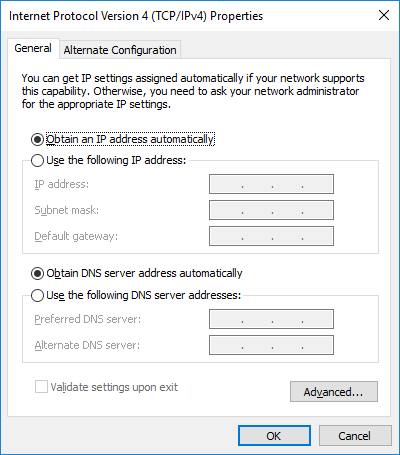
\includegraphics[width=0.6\textwidth]{chapters/11-net/img/windows-config.png}
  \caption{Configurarea rețelei în Windows}
  \label{fig:net:windows-config}
\end{figure}

În mod obișnuit, tipul de configurare (dinamică sau statică) este salvat în sistem; astfel că, la repornirea sistemului, configurația de rețea se menține.
Adică, în cazul configurării manuale salvate, se mențin parametrii de rețea, iar în cazul configurării automate salvate, se interoghează serverul DHCP la repornirea sistemului.
Este modul preferat de configurare pentru că, în general, ne dorim să menținem configurația la repornirea sistemului.

Pentru situații în care dorim să testăm configurații, sau pentru depanare, este util să realizăm \textbf{configurări temporare}, care pot fi ușor suprascrise și care nu se mențin la repornirea sistemului.

\section{Configurarea rețelei în Linux}
\label{sec:net:linux-config}

La fel ca în cazul celorlalte sisteme de operare, în Linux, investigarea parametrilor de rețea poate fi realizată de orice utilizator.
De cealaltă parte, configurarea parametrilor poate fi realizată doar de un utilizator cu permisiuni administrative (adică de contul \cmd{root} sau folosind \cmd{sudo} sau alte forme de obținere de privilegii administrative).
În mod tipic, utilizatorul implicit din interfața grafică de pe un sistem Linux are permisiuni de \cmd{sudo} și poate face astfel de operații.

\subsection{Inspectarea configurației}
\label{sec:net:linux-config:inspect}

Înainte de a realiza o configurație de rețea sau pentru a vedea că o configurație aplicată este corectă, un utilizator va inspecta configurația existentă.
Pentru depanarea problemelor, utilizatorul va verifica conectivitatea.
Am descris aceste acțiuni și modul de realizare a lor în Linux în \labelindexref{Secțiunea}{sec:net:config:interface}.
Sumarizăm mai jos cele mai frecvente acțiuni de inspectare a configurației și verificare a depanării:

\begin{itemize}
  \item listarea interfețelor și a configurației interfețelor de rețea (adresă MAC, adresă IP și mască):
    Folosim comanda \cmd{ip address show}, prezentată în \labelindexref{Listing}{lst:net:show-if-linux}.
  \item listarea tabelei de rutare (pentru aflarea adresei IP a gateway-ului):
    Folosim comanda \cmd{ip route show}: prezentată în \labelindexref{Listing}{lst:net:show-gateway}.
  \item afișarea serverelor DNS:
    Afișăm conținutul fișierului \file{/etc/resolv.conf}, prezentat în \labelindexref{Listing}{lst:net:show-dns}.
  \item verificarea conectivității:
    Folosim utilitarul \cmd{ping}, prezentat în \labelindexref{Listing}{lst:net:ping-positive}.
  \item verificarea funcționării serviciului DNS
    Folosim utilitarul \cmd{host}, prezentat în \labelindexref{Listing}{lst:net:check-dns}.
  \item verificarea ruterelor intermediare:
    Folosim utilitarul \cmd{traceroute}, prezentat în \labelindexref{Listing}{lst:net:check-route}.
  \item verificarea legăturii pe interfață:
    Folosim utilitarul \cmd{ethtool}, prezentat în \labelindexref{Listing}{lst:net:check-if}.
\end{itemize}

\subsection{Configurarea grafică. NetworkManager}
\label{sec:net:linux-config:gui}

Pe un sistem desktop un utilizator va folosi de obicei interfața grafică pentru a realiza configurarea rețelei.
Configurarea grafică este realizată în Linux cu ajutorul NetworkManager.
NetworkManager este un serviciu care permite configurarea facilă a interfeței în Linux.
Este compus dintr-un daemon care gestionează configurarea și interfețe grafice care facilitează configurarea, precum interfața din \labelindexref{Figura}{fig:net:nm-gui}.

\begin{figure}[!htbp]
  \centering
  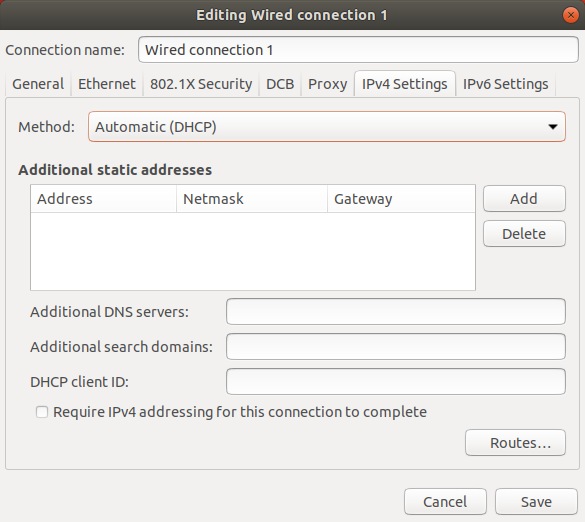
\includegraphics[width=0.8\textwidth]{chapters/11-net/img/nm-gui.png}
  \caption{Configurarea grafică a rețelei în Linux (NetworkManager)}
  \label{fig:net:nm-gui}
\end{figure}

Interfața din \labelindexref{Figura}{fig:net:nm-gui} poate fi pornită folosind comanda \cmd{nm-connection-editor}.
Configurarea realizată cu ajutorul NetworkManger poate fi statică sau dinamică.

Pe un sistem fără interfață grafică, avem diferite opțiuni de configurare a rețelei, opțiuni care sunt influențate și de distribuție.

\subsection{Configurarea DNS}
\label{sec:net:linux-config:dns}

În general, utilizatorul nu trebuie să fie preocupat de configurarea DNS.
Serverul DNS este, de obicei, obținut automat prin DHCP.
Într-un mediu desktop, NetworkManager se ocupă de configurarea DNS.

Pentru situații de depanare sau testare, un utilizator trebuie să aibă în vedere că DNS este configurat în fișierul \file{/etc/resolv.conf}, așa cum este exemplificat în \labelindexref{Listing}{lst:net:show-dns}.
În cadrul fișierului, serverele DNS (poate fi unul sau pot fi mai multe) sunt definite prin adresa IP pe liniile cu șirul \texttt{nameserver}.

În teorie, putem modifica sau adăuga noi servere DNS editând liniile cu șirul \texttt{nameserver} în fișierul \file{/etc/resolv.conf}.
Dar, pe majoritatea distribuțiilor Linux recente (cu sau fără interfața grafică), fișierul \file{/etc/resolv.conf} este editat periodic de managerul de rețea (precum NetworkManager) sau de alte utilitare care sunt apelate individual sau de manager: \cmd{resolvconf}, \cmd{systemd-resolved}, \cmd{dhclient}.
Modificările realizate în prealabil în fișier sunt suprascrise.
De aceea, dacă este nevoie să configurăm manual servere DNS pentru un sistem, va trebui să știm ce alte utilitare modifică fișierul \cmd{/etc/resolv.conf}.
Aceste utilitare vor suprascrie modificările manuale pe care le-am realizat.
Avem două opțiuni:
\begin{itemize}
  \item Configurăm respectivele utilitare (NetworkManager, \cmd{resolvconf}, \cmd{systemd-resolved}) pentru a putea configura serverele DNS.
    Nu mai edităm manual fișierul \file{/etc/resolv/conf}, ci configurăm utilitarele / serviciile respective.
    Configurarea poate înseamna editarea unor fișiere de configurare, specifice utilitarului.
  \item Dezactivăm respectivele utilitare sau le configurăm să nu modifice fișierul \cmd{/etc/resolv.conf}.
    Apoi putem să edităm manual fișierul \file{/etc/resolv.conf}.
\end{itemize}

Nu detaliem aici cum putem configura sau dezactiva utilitarele care editează fișierul \file{/etc/resolv.conf}.
Configurarea depinde de distribuție, de componentele instalate și de configurația sistemului.
Astfel de informații se pot găsi pe Internet\footnote{Modurile în care putem configura utilitarele să nu modifice fișierul \file{/etc/resolv.conf} sunt descrise aici: \url{https://www.ctrl.blog/entry/resolvconf-tutorial.html}}.

\subsection{Configurarea în linia de comandă}
\label{sec:net:linux-config:cli}

Atunci când sistemul dispune de interfață grafică, configurăm rețeaua folosind NetworkManager.
Configurarea în linia de comandă are loc pe acele sisteme în care nu avem interfață grafică.
În general, vom folosi linia de comandă și pe un sistem cu interfața grafică, dar mai degrabă pentru inspectarea configurației, așa cum am precizat în \labelindexref{Secțiunea}{sec:net:linux-config:inspect}.
Cazurile în care vom folosi linia de comandă pentru configurarea rețelei înt-run sistem cu interfață grafică sunt limitate.

Configurarea în linia de comandă poate fi realizată în mai multe moduri, depinzând de opțiunile utilizatorului și de distribuția folosită.
Unele metode sunt comune distribuțiilor, altele sunt specifice; fiecare distribuție oferă metode preferate de configurare.

\subsubsection{nmtui și nmcli}
\label{sec:net:linux-config:cli:nm}

Un prim mod de configurare a rețelei în linia de comandă, disponibil pe toate distribuțiile, este folosind utilitarele \cmd{nmtui} și \cmd{nmcli}, parte din NetworkManager.
\cmd{nmtui} oferă o interfață cu ferestre text pentru editarea configurației de rețea, ca în \labelindexref{Figura}{fig:net:nmtui}.
\cmd{nmcli} este folosit preponderent în forma cu argumente în linia de comandă pentru inspectarea și editarea configurației.
Cele două sunt utilitare de tip front end pentru serviciul NetworkManager, oferind aceleași opțiuni de configurare precum interfața grafică prezentată în \labelindexref{Figura}{fig:net:nm-gui}.

\begin{figure}[!htbp]
  \centering
  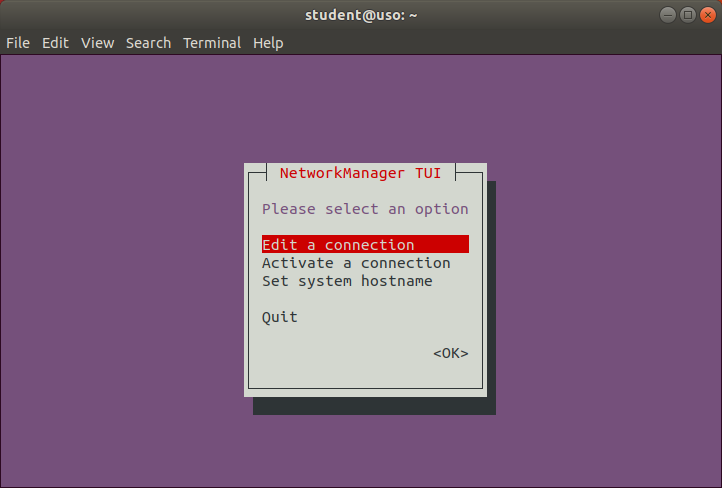
\includegraphics[width=0.8\textwidth]{chapters/11-net/img/nmtui.png}
  \caption{Configurarea rețelei în Linux folosind nmtui}
  \label{fig:net:nmtui}
\end{figure}

\subsubsection{Netplan (Ubuntu)}
\label{sec:net:linux-config:cli:netplan}

Pe distribuțiile Ubuntu recente (începând cu Ubuntu 18.04), configurarea rețelei în linia de comandă se realizează folosind Netplan\footnote{\url{https://netplan.io/}}.
Netplan oferă o interfață de fișiere de configurare în format YAML \abbrev{YAML}{YAML Ain't Markup Language} (\textit{YAM Ain't Markup Language}).
Utilizatorul / administratorul editează aceste fișiere de configurare, apoi aplică acea configurație.
Aplicarea configurației duce la stabilirea parametrilor de rețea.
Pasul de aplicare se realizează prin intermediul unui \textit{renderer}.
În mod implicit rendererul este NetworkManager.

Configurația Netplan implicită pe o instalare Ubuntu 18.04 cu interfață grafică este cea din fișierul \texttt{/etc/netplan/01-network-manager-all.yaml}, indicat în \labelindexref{Listing}{lst:net:netplan-default}.

\begin{screen}[caption={Configure implicită},label={lst:net:netplan-default}]
student@uso:~$ cat /etc/netplan/01-network-manager-all.yaml
# Let NetworkManager manage all devices on this system
network:
  version: 2
    renderer: NetworkManager
\end{screen}

Dacă dorim o configurație specifică pentru interfața \texttt{enp0s3}, vom folosi un conținut precum cel din \labelindexref{Listing}{lst:net:netplan-static}.
Folosind comanda \cmd{netplan try} (linia \texttt{14}), am verificat validitatea conținutului fișierului de configurare.
Și, folosind \cmd{netplan apply} (linia \texttt{24}), am aplicat configurația.

\begin{screen}[caption={Configure implicită},label={lst:net:netplan-static}]
student@uso:~$ cat /etc/netplan/01-network-manager-all.yaml
# Let NetworkManager manage all devices on this system
network:
  version: 2
  renderer: NetworkManager
  ethernets:
    enp0s3:
      addresses:
        - 192.168.0.7/24
      gateway4: 192.168.0.1
      nameservers:
        addresses: [8.8.8.8, 4.4.4.4]

student@uso:~$ sudo netplan try
Do you want to keep these settings?


Press ENTER before the timeout to accept the new configuration


Changes will revert in 119 seconds
Configuration accepted.

student@uso:~$ sudo netplan apply

student@uso:~$ ip a s enp0s3
2: enp0s3: <BROADCAST,MULTICAST,UP,LOWER_UP> mtu 1500 qdisc fq_codel state UP group default qlen 1000
    link/ether 08:00:27:3a:a9:01 brd ff:ff:ff:ff:ff:ff
    inet 192.168.0.7/24 brd 192.168.0.255 scope global noprefixroute enp0s3
       valid_lft forever preferred_lft forever
    inet6 fe80::a00:27ff:fe3a:a901/64 scope link
       valid_lft forever preferred_lft forever

student@uso:~$ ip r s
default via 192.168.0.1 dev enp0s3 proto static metric 20100
192.168.0.0/24 dev enp0s3 proto kernel scope link src 192.168.0.7 metric 100
192.168.56.0/24 dev enp0s8 proto kernel scope link src 192.168.56.101 metric 101
\end{screen}

Informații extinse despre configurarea rețelei în linia de comandă în Ubuntu se găsesc în documentația oficială (\url{https://ubuntu.com/server/docs/network-configuration}).

\subsubsection{ifupdown (Debian / Ubuntu)}
\label{sec:net:linux-config:cli:ifupdown}

Modul clasic de configurare în linia de comandă în distribuțiile Debian / Ubuntu este folosind pachetul \texttt{ifupdown}.
În distribuțiile mai noi Ubuntu, se preferă folosirea Netplan.
În distribuțiile Debian mai noi, se preferă folosirea Systemd-Networkd\footnote{\url{https://wiki.debian.org/SystemdNetworkd}}.

În cazul folosirii \texttt{ifupdown}, configurațiile de rețea se rețin în fișiere din directorul \file{/etc/network/}.
Configurațiile fundamentale de rețea se rețin în fișierul \file{/etc/network/interfaces}.
\labelindexref{Listing}{lst:net:ifupdown} conține un exemplu de configurație a interfeței \texttt{eth0}.
Linia \texttt{2} se precizează că este vorba de o configurație statică a interfeței.
Apoi se precizează adresa IP (inclusiv masca) și gateway-ul.

\begin{screen}[caption={Configurație ifupdown în /etc/network/interfaces},label={lst:net:ifupdown}]
auto eth0
iface eth0 inet static
	address 192.168.0.7/24
	gateway 192.168.0.1
\end{screen}

Configurațiile sunt aplicate cu ajutorul comenzilor \cmd{ifup} și \cmd{ifdown}.
Aceste comenzi sunt invocate pentru aplicarea configurației din fișierul \cmd{/etc/network/interfaces}.
\cmd{ifup} activează configurația și interfața, în vreme ce \cmd{ifdown} deconfigurează și dezactivează interfața.
Ambele comenzi pot primi ca parametru numele interfeței, sau pot primi opțiunea \texttt{-a}, caz în care se aplică pe toate interfețele marcate cu \texttt{auto} în fișierul \file{/etc/network/interfaces}, cum este și cazul liniei \texttt{1} din \labelindexref{Listing}{lst:net:ifupdown}.

\texttt{ifupdown} poate coexista cu NetworkManager.
În configurația implicită a NetworkManager, orice interfețe prezente în fișierul \file{/etc/network/interfaces} sunt excluse din configurația NetworkManager.

Informații extinse despre configurarea rețelei în Debian se găsesc în documentația oficială (\url{https://wiki.debian.org/NetworkConfiguration}, \url{https://www.debian.org/doc/manuals/debian-reference/ch05.en.html}).

\subsection{ifcfg (Fedora / RedHat)}
\label{sec:net:linux-config:cli:ifcfg}

Modul clasic de configurare în linia de comandă în distribuțiile Fedora / Redhat este folosind \texttt{ifcfg}.
Similar Netplan și \texttt{ifupdown}, \texttt{ifcfg} presupune realizarea de configurații în fișiere specifice.

Configurațiile se realizează, de regulă, în fișiere din directorul \file{/etc/sysconfig/network-scripts/}.
Dacă dorim să configurăm interfața \texttt{enp0s3} vom crea și edita fișierul \file{/etc/sysconfig/network-scripts/ifcfg-enp0s3}, ca în \labelindexref{Listing}{lst:net:ifcfg}.
Configurația conține linii de forma \verb|<cheie>=<valoare>|.
De exemplu, \texttt{DEVICE} va retine numele interfeței, \texttt{BOOTPROTO} tipul configurației, \texttt{IPADDR} adresa IP, iar \texttt{GATEWAY} adresa IP a gateway-ului.

\begin{screen}[caption={Configurație ifcfg},label={lst:net:ifcfg}]
[student@uso:~]$ cat /etc/sysconfig/network-scripts/ifcfg-enp0s3
DEVICE=enp0s3
TYPE=Ethernet
BOOTPROTO=non
NAME=enp0s3
ONBOOT=yes
PREFIX=24
IPADDR=192.168.0.7
GATEWAY=192.168.0.1
\end{screen}

Activarea și dezactivarea configurației se realizează cu ajutorul serviciului de networking folosind comenzi precum \cmd{sudo service network start}, \cmd{sudo service network stop}, \cmd{sudo service network restart}.
Dacă pe sistem rulează NetworkManager, atunci putem dezactiva NetworkManager la nivelul interfeței.
Pentru aceasta, în fișierul de configurare al intefeței (de exemplu \file{/etc/sysconfig/network-scripts/ifcfg-eth0}), adăugăm linia de configurare \verb|NM_CONTROLLED=no|.

Informații extinse despre configurarea rețelei în Fedora / RedHat se găsesc în documentația Fedora (\url{https://docs.fedoraproject.org/en-US/Fedora/25/html/Networking\_Guide/ch-Configure\_Networking.html}, \url{https://access.redhat.com/documentation/en-us/red\_hat\_enterprise\_linux/7/html/networking\_guide/ch-configuring\_ip\_networking}).

\subsection{Interfețe active/inactive}
\label{sec:net:linux-config:up-down-if}

Pentru a putea folosi o configurație, interfața corespunzătoare trebuie să fie activă.
Pentru a activa, dezactiva și verifica o interfață folosim comanda ip link ca în \labelindexref{Listing}{lst:net:enable-if}.

Folosim comanda \cmd{ip link show} pentru a afișa informații despre legătura interfețelor sistemului: dacă sunt active, adresa MAC, unitatea de transmitere (MTU - \textit{Maximum Transmission Unit}) etc.
În mod implicit se afișează informații despre toate interfețele sistemului (liniile \texttt{1-7});
se pot afișa informații despre o singură interfață prin transmiterea numelui acelei interfețe ca argument (liniile \texttt{11-13} și \texttt{17-19}).
Atunci când rezultatul rulării comenzii de afișare conține șirul \textit{state UP}, interfața este activă; altfel, dacă șirul conținut este \textit{state DOWN}, interfața este inactivă.
Folosind comanda \cmd{ip link set dev enp0s3 down} (în mod privilegiat, linia \texttt{10}) dezactivăm interfața \texttt{enp0s3}, iar folosind comanda \cmd{ip link set dev eth0 up} (în mod privilegiat, linia \texttt{15}) activăm interfața.
Apoi starea interfeței va fi actualizată în \texttt{DOWN}, respectiv \texttt{UP}, în rezultatul rulării comenzi ip link show.

\begin{screen}[caption={Activarea și dezactivarea unei interfețe},label={lst:net:enable-if}]
student@uso:~$ ip link show
1: lo: <LOOPBACK,UP,LOWER_UP> mtu 65536 qdisc noqueue state UNKNOWN mode DEFAULT group default qlen 1000
    link/loopback 00:00:00:00:00:00 brd 00:00:00:00:00:00
2: enp0s3: <BROADCAST,MULTICAST,UP,LOWER_UP> mtu 1500 qdisc fq_codel state UP mode DEFAULT group default qlen 1000
    link/ether 08:00:27:3a:a9:01 brd ff:ff:ff:ff:ff:ff
3: enp0s8: <BROADCAST,MULTICAST,UP,LOWER_UP> mtu 1500 qdisc fq_codel state UP mode DEFAULT group default qlen 1000
    link/ether 08:00:27:c0:83:50 brd ff:ff:ff:ff:ff:ff

student@uso:~$ sudo ip link set dev enp0s3 down

student@uso:~$ ip link show enp0s3
2: enp0s3: <BROADCAST,MULTICAST> mtu 1500 qdisc fq_codel state DOWN mode DEFAULT group default qlen 1000
    link/ether 08:00:27:3a:a9:01 brd ff:ff:ff:ff:ff:ff

student@uso:~$ sudo ip link set dev enp0s3 up

student@uso:~$ ip link show enp0s3
2: enp0s3: <BROADCAST,MULTICAST,UP,LOWER_UP> mtu 1500 qdisc fq_codel state UP mode DEFAULT group default qlen 1000
    link/ether 08:00:27:3a:a9:01 brd ff:ff:ff:ff:ff:ff
\end{screen}

\subsection{Configurarea temporară. Comanda ip}
\label{sec:net:linux-config:temporary}

Configurarea temporară în Linux se realizează în linia de comandă și este universală pe toate tipurile de distribuții.
Configurarea temporară se realizează cu ajutorul utilitarul \cmd{ip}.
Am folosit utilitarul \cmd{ip} în \labelindexref{Secțiunea}{sec:net:config:interface} pentru investigarea configurației și în \labelindexref{Secțiunea}{sec:net:linux-config:up-down-if} pentru activarea / dezactivarea unei interfețe.

Comenzile de configurare a interfețelor de rețea sunt comenzi privilegiate.
De aceea, în secvențele de comenzi pe care le vom prezenta, acestea sunt prefixate de comanda \cmd{sudo}.

Înainte de a configura temporar parametrii de rețea, se recomandă să se șteargă configurațiile anterioare.
Acest lucru poate fi făcut cu ajutorul comenzii \cmd{ip address flush}, ca în \labelindexref{Listing}{lst:net:flush-if}.
După rularea comenzii \cmd{ip address flush} (în mod privilegiat), orice configurații anterioare ale interfeței sunt șterse.

\begin{screen}[caption={Ștergerea configurațiilor unei interfețe},label={lst:net:flush-if}]
student@uso:~$ ip address show enp0s3
2: enp0s3: <BROADCAST,MULTICAST,UP,LOWER_UP> mtu 1500 qdisc fq_codel state UP group default qlen 1000
    link/ether 08:00:27:3a:a9:01 brd ff:ff:ff:ff:ff:ff
    inet 10.0.2.15/24 brd 10.0.2.255 scope global dynamic noprefixroute enp0s3
       valid_lft 76576sec preferred_lft 76576sec

student@uso:~$ sudo ip address flush enp0s3

student@uso:~$ ip address show enp0s3
2: enp0s3: <BROADCAST,MULTICAST,UP,LOWER_UP> mtu 1500 qdisc fq_codel state UP group default qlen 1000
    link/ether 08:00:27:3a:a9:01 brd ff:ff:ff:ff:ff:ff
\end{screen}

Pentru configurarea unei adrese IP și a unei măști pe o interfață folosim comanda \cmd{ip address add}.
În \labelindexref{Listing}{lst:net:add-ip} avem exemple de configurare a adresei IP \cmd{192.168.0.7/24} pe interfața \texttt{enp0s3}.
În prelabil, am șters configurația interfeței \texttt{enp0s3} folosind comanda \cmd{ip address flush}.

\begin{screen}[caption={Configurarea unei adrese pe o interfață},label={lst:net:add-ip}]
student@uso:~$ sudo ip address flush enp0s3

student@uso:~$ ip address show enp0s3
2: enp0s3: <BROADCAST,MULTICAST,UP,LOWER_UP> mtu 1500 qdisc fq_codel state UP group default qlen 1000
    link/ether 08:00:27:3a:a9:01 brd ff:ff:ff:ff:ff:ff

student@uso:~$ sudo ip address add 192.168.0.7/24 dev enp0s3
student@uso:~$ ip address show enp0s3
2: enp0s3: <BROADCAST,MULTICAST,UP,LOWER_UP> mtu 1500 qdisc fq_codel state UP group default qlen 1000
    link/ether 08:00:27:3a:a9:01 brd ff:ff:ff:ff:ff:ff
    inet 192.168.0.7/24 scope global enp0s3
       valid_lft forever preferred_lft forever
\end{screen}

Comanda \cmd{ip address add}, așa cum îi spune numele, adaugă o nouă adresă IP interfeței de rețea.
O interfață de rețea poate avea astfel mai multe adrese IP.
În \labelindexref{Listing}{lst:net:del-ip}, ștergem toate configurația pe interfața de rețea \texttt{enp0s3} (linia \texttt{1}), adăugăm două adrese IP pe o interfață de rețea (liniile \texttt{7-9}) și apoi o ștergem pe una dintre ele folosind comanda \cmd{ip address del} (linia \texttt{19}).

\begin{screen}[caption={Ștergerea unei adrese de pe o interfață},label={lst:net:del-ip}]
student@uso:~$ sudo ip address flush enp0s3

student@uso:~$ ip address show enp0s3
2: enp0s3: <BROADCAST,MULTICAST,UP,LOWER_UP> mtu 1500 qdisc fq_codel state UP group default qlen 1000
    link/ether 08:00:27:3a:a9:01 brd ff:ff:ff:ff:ff:ff

student@uso:~$ sudo ip address add 192.168.0.7/24 dev enp0s3

student@uso:~$ sudo ip address add 172.16.19.7/24 dev enp0s3

student@uso:~$ ip address show enp0s3
2: enp0s3: <BROADCAST,MULTICAST,UP,LOWER_UP> mtu 1500 qdisc fq_codel state UP group default qlen 1000
    link/ether 08:00:27:3a:a9:01 brd ff:ff:ff:ff:ff:ff
    inet 192.168.0.7/24 scope global enp0s3
       valid_lft forever preferred_lft forever
    inet 172.16.19.7/24 scope global enp0s3
       valid_lft forever preferred_lft forever

student@uso:~$ sudo ip address del 172.16.19.7/24 dev enp0s3

student@uso:~$ ip address show enp0s3
2: enp0s3: <BROADCAST,MULTICAST,UP,LOWER_UP> mtu 1500 qdisc fq_codel state UP group default qlen 1000
    link/ether 08:00:27:3a:a9:01 brd ff:ff:ff:ff:ff:ff
    inet 192.168.0.7/24 scope global enp0s3
       valid_lft forever preferred_lft forever
\end{screen}

Pentru configurarea gateway-ului folosim comanda \cmd{ip route add default}.
În mod similar, dacă dorim să ștergem configurația gateway-ului folosim comanda \cmd{ip route del}.
În \labelindexref{Listing}{lst:net:add-gw} avem exemplu de configurare a gateway-ului cu adresa IP \cmd{192.168.0.1}.

\begin{screen}[caption={Configurarea gateway-ului},label={lst:net:add-gw}]
student@uso:~$ ip route show
192.168.0.0/24 dev enp0s3 proto kernel scope link src 192.168.0.7
192.168.56.0/24 dev enp0s8 proto kernel scope link src 192.168.56.101

student@uso:~$ sudo ip route add default via 192.168.0.1

student@uso:~$ ip route show
default via 192.168.0.1 dev enp0s3
192.168.0.0/24 dev enp0s3 proto kernel scope link src 192.168.0.7
192.168.56.0/24 dev enp0s8 proto kernel scope link src 192.168.56.101
\end{screen}

Adresa IP a gateway-ului trebuie să se găsească în rețeaua locală, adică să fie similară cu adresele IP configurate pe interfețe.
Dacă încercăm să configurăm pentru gateway o adresă IP care nu este în rețeaua locală, primim o eroare precum cea din \labelindexref{Listing}{lst:net:add-gw-err}: \textit{Nexthop has invalid gateway}.

\begin{screen}[caption={Configurare gateway-ului cu adresă IP nevalidă},label={lst:net:add-gw-err}]
student@uso:~$ ip route show
192.168.0.0/24 dev enp0s3 proto kernel scope link src 192.168.0.7 
192.168.56.0/24 dev enp0s8 proto kernel scope link src 192.168.56.101 

student@uso:~$ sudo ip route add default via 68.212.2.1
Error: Nexthop has invalid gateway.
\end{screen}

\subsection{Configurarea DHCP. Comanda dhclient}
\label{sec:net:dhclient}

Configurările de mai sus sunt configurări manuale, cu adresele precizate de utilizator.
Dacă dorim să configurăm parametrii de rețea în mod automat, interogând serverul DHCP al rețelei locale, folosim clientul DHCP dat de utilitarul \cmd{dhclient}, ca în \labelindexref{Listing}{lst:net:dhclient}.
Rularea comenzii \cmd{dhclient} duce la configurarea tuturor parametrilor de rețea furnizați prin DHCP: adresă IP, mască de rețea, gateway, server DNS.
Am folosit în prealabil comanda \cmd{ip address flush} ca să ștergem configurația interfeței \texttt{enp0s3}.

\begin{screen}[caption={Configurarea automată (prin DHCP) din linia de comandă},label={lst:net:dhclient}]
student@uso:~$ sudo ip address flush enp0s3

student@uso:~$ ip address show enp0s3
2: enp0s3: <BROADCAST,MULTICAST,UP,LOWER_UP> mtu 1500 qdisc fq_codel state UP group default qlen 1000
    link/ether 08:00:27:3a:a9:01 brd ff:ff:ff:ff:ff:ff

student@uso:~$ ip route show
192.168.56.0/24 dev enp0s8 proto kernel scope link src 192.168.56.101 

student@uso:~$ sudo dhclient enp0s3

student@uso:~$ ip address show enp0s3
2: enp0s3: <BROADCAST,MULTICAST,UP,LOWER_UP> mtu 1500 qdisc fq_codel state UP group default qlen 1000
    link/ether 08:00:27:3a:a9:01 brd ff:ff:ff:ff:ff:ff
    inet 10.0.2.15/24 brd 10.0.2.255 scope global enp0s3
       valid_lft forever preferred_lft forever

student@uso:~$ ip route show
default via 10.0.2.2 dev enp0s3
10.0.2.0/24 dev enp0s3 proto kernel scope link src 10.0.2.15
192.168.56.0/24 dev enp0s8 proto kernel scope link src 192.168.56.101
\end{screen}

\subsection{Sumar}
\label{sec:net:linux-config:summary}

În Linux, pentru configurarea rețelei, folosim, în general, interfața grafică.
Interfața grafică folosește un serviciu de rețea (NetworkManager).

Configurarea în linia de comandă poate fi realizată în mai multe moduri, depinzând de opțiunile utilizatorului și de distribuția folosită.
Configurarea în linia de comandă se face folosind fișiere de configurare.
Opțiuni pentru configurarea în linia de comandă sunt Netplan (Ubuntu), \texttt{ifupdown} (Debian / Ubuntu), \texttt{ifcfg} (RedHat).

Pentru diagnosticare, testare sau depanare putem folosi configuare temporară.
Configurarea temporară se realizează cu ajutorul utilitarul \cmd{ip}.

\section{Aplicații de rețea. Webul}
\label{sec:net:apps}

Odată configurat accesul la Internet al unei stații (sistem, dispozitiv), utilizatorul poate accesa servicii din Internet: conținut media, rețele sociale, medii de stocare, soluții colaborative, comunicare online, acces la distanță.
Pentru accesarea acestor servicii, utilizatorul folosește aplicații specializate numite aplicații client.
O aplicație client este un proces care rulează pe stația locală care folosește un protocol cunoscut pentru a se conecta, prin Internet, la o aplicație server (sau serviciu).
Aplicația server este un proces care rulează pe un sistem server și oferă servicii în Internet, servicii ce sunt accesate de utilizatori prin aplicațiile client.
De exemplu, atunci când folosim pe un dispozitiv mobil aplicația client WhatsApp, aceasta se va conecta la o aplicația server furnizată de compania Facebook și va putea interacționa cu alte aplicații WhatsApp de pe alte dispozitive.
La fel, pe un sistem desktop folosim aplicația client Dropbox, care se va conecta la o aplicație server Dropbox pentru a sincroniza fișierele locale cu cele de la distanță.

În vreme ce pe dispozitivele mobile sau de tip smart TV există este uzual să existe aplicații client dedicate pentru fiecare tip de serviciu (YouTube, Facebook, WhatsApp, Google Hangouts, Google Drive, Maps, Calendar, Mail), pe sistemele desktop multe dintre aceste servicii sunt accesate printr-un navigator (browser) web.
Un browser web este un client web (sau client HTTP).
Întrucât multe dintre serviciile din Internet sunt accesate prin web / HTTP, un browser web poate fi folosit în rol de client generic.
Un browser web poate fi folosit și pe dispozitivele mobile sau smart TV, dar, uzual, există o aplicație dedicată care facilitează accesul serviciului.
La fel și pe sistemele desktop: pot exista aplicații dedicate (precum un client Google Drive sau un client de e-mail precum Microsoft Outlook sau Mozilla Thunderbird), dar mulți utilizatori preferă folosirea unei interfețe unice dată de clientul web.

Abordarea folosirii unei aplicații dedicate are avantajul unui acces mai rapid al serviciului: se pornește aplicația și, dacă este configurația realizată, accesează serviciul.
De cealaltă parte, avantajul folosirii unui browser web înseamnă că furnizorul serviciului nu trebuie să mai dezvolte o aplicație client dedicată, ci să se concentreze doar pe implementarea serviciului.
De asemenea, utilizatorul serviciului nu are nevoie să instaleze o aplicație dedicată, ci folosește browser-ul web pe care îl întâlnește pe orice sistem;
poate folosi inclusiv browserul web pe un sistem străin, unde probabil nu are permisiuni de instalare.
Browserul web devine astfel una dintre aplicațiile esențiale ale sistemelor conectate la Internet.
Browserele web moderne (Safari, Microsoft Edge, Mozilla Firefox) sunt aplicații complexe, cu funcționalități care să permită o experiență cât mai plăcută și performantă utilizatorului care va accesa servicii din Internet.

\subsection{Serviciul web}
\label{sec:net:apps:web}

Browserele sunt clienți web care folosesc protocolul HTTP (\textit{Hypertext Transfer Protocol}) pentru accesarea serviciilor expuse.
Popularitatea webului și a protocolui HTTP a dus la situația în care furnizorii de servicii de Internet își proiectează serviciile direct să fie accesate prin HTTP, sau să ofere și această interfață.
De exemplu, Netflix permite vizualizarea de filme prin intermediul protocolului HTTP, fie din aplicație dedicată (pe un smart TV), fie printr-un browser web.

Protocolul HTTP este în esență un protocol de acces de resurse de la distanță.
Pentru accesarea acestor resurse, este nevoie de un mod de identificare a acestora, o adresă.
Acest identificator este URL (\textit{Uniform Resource Locator}), numit și adresă web.
Este acea adresă pe care o introducem în bara de adrese a unui browser web.
Un URL este compus din trei elemente:
\begin{itemize}
  \item protocolul folosit: uzual HTTP sau HTTPs (HTTP securizat)
  \item numele sistemului pe care rulează serviciul: uzual este un nume DNS (precum \texttt{google.com}), dar poate fi și o adresă IP
  \item calea către resursă: modul în care serviciul web localizează pe server resursa.
    Resursa este uzual o pagină web.
    Pagina web este transferată de la serviciul web la clientul web (browser) unde este redată (\textit{rendered}) în ceea ce vede la final utilizator.
\end{itemize}

De exemplu, în cadrul URL-ului \url{https://ocw.cs.pub.ro/courses/uso/cursuri/curs-05}, protocolul este \texttt{https}, numele sistemului este \texttt{ocw.cs.pub.ro}, iar calea către resursă (adică pagina web aferentă cursului 5 de USO) este \texttt{courses/uso/cursuri/curs-05}.

Folosim un browser web pentru accesarea unor servicii de la distanță, cel mai adesea în formă de pagini web care for redate de browser.
Pentru cazul în care dorim descărcarea unei resurse, sau accesarea unui serviciu simplu sau pentru automatizare sau testare putem folosi utilitare de tip clienți web în linia de comandă.
Cele mai întâlnite astfel de utilitare în Linux sunt \cmd{wget} sau \cmd{curl}.
Cele două au funcționalități similare, numai că, implicit, \cmd{wget} salvează conținutul de la URL transmis ca argument într-un fișier, în vreme ce \cmd{curl} afișează conținutul la ieșirea standard.
O altă diferență este că \cmd{wget} permite descărcarea recursivă a resurselor; adică linkurile web sunt accesate și apoi se realizează transferul și resurselor respective.
\cmd{wget} folosește protocoalele HTTP, HTTPS, FTP; \cmd{curl} adaugă suport și pentru alte protocoale.
Câteva exemple de funcționare sunt în \labelindexref{Listing}{lst:net:wget-curl}.

\begin{screen}[caption={Clienți web în linie de comandă: wget și curl},label={lst:net:wget-curl}]
student@uso:~$ wget http://acs.pub.ro/~cpop/orare_sem1/Orar1CD.xls
--2021-01-16 13:24:51--  http://acs.pub.ro/~cpop/orare_sem1/Orar1CD.xls
Resolving acs.pub.ro (acs.pub.ro)... 141.85.227.151
[...]
2021-01-16 13:24:51 (1.39 MB/s) - 'Orar1CD.xls' saved [50688/50688]

student@uso:~$ curl icanhazip.com
95.76.43.212

student@uso:~$ wget --user <username> --ask-pass https://repository.grid.pub.ro/cs/uso/USO.ova
Password for user '<username>':
--2021-01-16 13:26:04--  https://repository.grid.pub.ro/cs/uso/USO.ova
Resolving repository.grid.pub.ro (repository.grid.pub.ro)... 141.85.241.222
[...]
Saving to: 'USO.ova'
\end{screen}

\subsection{Alte servicii}
\label{sec:net:apps:other}

Unele servicii nu sunt accesate prin web / HTTP, ci prin alte protocoale, sau și prin alte protocoale.
În această situație, există aplicații client dedicate pentru accesarea serviciilor.
Exemple de astfel de servicii sunt conexiune la distanță, poștă electronică și transfer de fișiere.

\subsubsection{Conexiune la distanță}
\label{sec:net:apps:other:remote}

Conexiunea la distanță (\textit{remote connection}) permite accesarea și controlul unui sistem din Internet de pe o stație locală.
Prin canalul de comunicație realizat între stația locală și sistemul de la distanță pot fi trimise comenzi.
Interacțiunea cu sistemul aflat la distanță poate fi cu interfață grafică (serviciu numit și \textit{remote desktop} / \textit{desktop sharing}) sau interfață în linie de comandă (serviciu numit și \textit{remote shell}).
Dat fiind că este sensibilă oferirea accesului la un sistem, serviciile de conexiune la distanță au integrate componente de autentificare și confidențialitate.

Microsoft a dezvoltat protocolul RDP \abbrev{RDP}{Remote Desktop Protocol} (\textit{Remote Desktop Protocol}) pentru conexiunea la distanță cu interfață grafică;
serviciul RDP este încorporat în sistemul de operare Windows.
RDP este folosit în principal pentru Windows, dar există aplicații client și server pentru alte sisteme de operare.

O aplicație de tipul \textit{remote desktop} este TeamViewer.
Aplicația acționează simultan în rol de server și de client.
Un utilizator care instalează aplicația pe sistem propriu o poate folosi pentru a se conecta la alte sisteme, sau pentru a permite altor utilizatori să se conecteze la sistemul său.
O aplicație similară este AnyDesk.

VNC \abbrev{VNC}{Virtual Network Computing} (\textit{Virtual Network Computing}) este un alt sistem de tipul \textit{desktop sharing}.
Cuprinde un server VNC, un client VNC și protocolul RFB \abbrev{RFB}{Remote Frame Buffer} (\textit{Remote Frame Buffer}) folosit pentru comunicare.

Pentru acces la distanță în linia de comandă, cel mai întâlnit protocol este SSH (\textit{Secure Shell}).
Protocolul SSH creează un canal sigur de comunicare (criptat).
În acest canal se poate opta pentru deschiderea unei sesiuni shell la distanță (\textit{remote shell}) sau pentru transfer de fișier sau pentru tunelarea altor protocoale pentru a le adăuga funcționalități de securitate.
Ca să deschidem o sesiune shell la distanță folosim, în Linux, comanda \cmd{ssh} urmată de numele de cont (\textit{username}) și numele stației, ca în \labelindexref{Listing}{lst:net:ssh}.

\begin{screen}[caption={Conexiune la distanță folosind SSH},label={lst:net:ssh}]
student@uso:~$ whoami
student
student@uso:~$ hostname
uso
razvan@jotunn:~$ ssh asm@elf.cs.pub.ro
Linux elf 2.6.32-5-amd64 #1 SMP Tue May 13 16:34:35 UTC 2014 x86_64
[...]
asm@elf:~$ whoami
asm
asm@elf:~$ hostname
elf
\end{screen}

În \labelindexref{Listing}{lst:net:ssh}, ne-am conectat de pe sistemul cu numele \texttt{uso}, din contul \texttt{student}, pe sistemul cu numele \texttt{elf.cs.pub.ro} în contul \texttt{uso}.
Avem deschisă o sesiune shell la distanță unde putem rula comenzi și unde putem administra sistemul.

În sistemele Linux, pentru administrarea sistemelor și data centerelor, se folosește aproape exclusiv protocolul SSH.
Mai multe detalii despre protocolul SSH vom prezenta în \labelindexref{Secțiunea}{sec:sec:transfer:ssh}.

\subsubsection{E-mail}
\label{sec:net:apps:other:e-mail}

Serviciul de poștă electronică (e-mail) este folosit pentru transmisia de mesaje între utilizatori.
Fiecare utilizator dispune de o căsuță poștală electronică (\textit{electronic mailbox}) unde primește mesajele.
Pentru accesarea căsuței poștale și pentru trimiterea de mesaje (e-mailuri), folosește protocoale specifice serviciului de e-mail și un client de e-mail care cunoaște aceste protocoale.
Exemple de clienți de e-mail sunt Microsoft Outlook sau Mozilla Thunderbird.
Aceștia se conectează la servere de e-mail corespunzătoare pentru a citi și a trimite mesaje.

Așa cum am precizat mai sus, multe servicii sunt interfațate prin web.
Astfel, și furnizorii de servicii de e-mail oferă, în general, o interfața web care acționează ca un client de e-mail.
Este exemplul serviciilor GMail sau ProtonMail care sunt accesate dintr-un browser web.

Serviciul de poștă electronică este similar cu serviciile de mesagerie (\textit{instant messaging}) precum WhatsApp, Facebook Messenger, Telegram, Signal.
O bună parte dintre utilizatori preferă folosirea acestor servicii de mesagerie pentru comunicare mai rapidă și creare facilă de grupuri de lucru și conferințe audio și video.
Cu toate acestea, serviciul de e-mail rămâne util din câteva motive:
\begin{itemize}
  \item Are o organizare și accesare mai bună a mesajelor (în căsuța poștală).
  \item Este de așteptat să nu primească un răspuns imediat.
  \item Este mai adecvat mediilor profesionale, în care legăturile sunt mai formale.
  \item Pentru că permite construcția de liste sau grupuri de discuții cu arhive de mesaje care pot fi consultate ulterior.
\end{itemize}

\subsubsection{Transfer de fișiere}
\label{sec:net:apps:other:file-transfer}

Transferul de fișiere, după cum îi spune și numele, este un serviciu care permite transmiterea fișierelor (datelor) între o sursă și destinație.
Fundamental, protocolul HTTP (\textit{Hypertext Transfer Protocol}), așa cum îi spune și numele, este un protocol de transfer de date.

Protocolul HTTP are utilizări care pot fi mai degrabă clasificate ca fiind acces la distanță, în vreme ce alte protocoale sunt folosite exclusiv pentru transferul de fișiere.
Deși poate face și încărcare de informații (\textit{upload}), protocolul HTTP este folosit, în general, pentru descărcare (\textit{download}).

Protocolul SSH (\textit{Secure Shell}) de care am amintit mai sus permite transferul de fișiere în formă securizată.
Atunci când avem un cont pe un sistem la distanță este forma preferată de transfer de fișiere.

Protocolul FTP \abbrev{FTP}{File Transfer Protocol} (\textit{File Transfer Protocol}) are ca rol transferul fișierelor.
Spre deosebire de HTTP, protocolul FTP permite mai ușor încărcarea de fișiere (\textit{upload}).
Spre deosebire de SSH, protocolul nu necesită un cont la distanță.
De aceea, este protocolul preferat folosit de furnizorii de servicii de găzduire (\textit{hosting services}) care nu doresc, din rațiuni de securitate, să ofere un cont pentru acces la distanță.

Pentru transferul de date în rețele mai mari de noduri (numite \textit{swarmuri}) folosim protocolul BitTorrent.
Protocolul BitTorrent este un protocol peer-to-peer, în care fiecare nod este simultan și client și server, permițând și descărcarea (\textit{download}) și încărcarea (\textit{upload}) de informații.
Este în special util pentru distribuția de fișiere de mari dimensiuni.
În perioada 2005-2010 transferurile prin BitTorrent erau printre cele mai consumatoare de lățime de bandă din Internet, în special pentru conținut video, adesea piratat.
Între timp, dezvoltarea infrastructurii de Internet și popularitatea serviciilor de video streaming precum YouTube sau Netflix, au dus la diminuarea folosirii BitTorrent.

\section{Anexă: Configurări de rețea folosind suita ifconfig/route}
\label{sec:net:config-ifconfig}

Pe sistemele Linux folosim suita \cmd{iproute2} (care conține utilitarul \cmd{ip}) pentru investigarea și configurarea rețelei în linia de comandă.
Până la apariția \cmd{iproute2}, aceste acțiuni erau realizate cu utilitare precum \cmd{ifconfig} și \cmd{route}.
Aceste utilitare pot fi, în continuare, folosite în Linux, deși preferăm suita \cmd{iproute2} care are un număr mai mare de funcționalități.

Un avantaj al cunoașterii utilitarelor de forma \cmd{ifconfig} și \cmd{route} este că sunt prezente pe toate sistemele din familia Unix.
Dacă vom avea de-a face cu sisteme rulând FreeBSD sau macOS, vom putea folosi \cmd{ifconfig} și \cmd{route} pentru configurarea rețelei.

Folosim \cmd{ifconfig} pentru a afișa informații despre interfețele de rețea și folosim \cmd{route} pentru a afișa tabela de rutare, incluzând gateway-ul, ca în \labelindexref{Listing}{lst:net:show-ifconfig-route}.
Comanda \cmd{ifconfig} afișează implicit doar interfețele active.
Dacă dorim să afișăm informații despre toate interfețele (active și inactive) folosim opțiunea \cmd{-a} la comanda \cmd{ifconfig} (liniile \texttt{20-45}).

\begin{screen}[caption={Vizualizarea parametrilor de rețea cu ifconfig/route},label={lst:net:show-ifconfig-route}]
student@uso:~$ ifconfig
enp0s8: flags=4163<UP,BROADCAST,RUNNING,MULTICAST>  mtu 1500
        inet 192.168.56.101  netmask 255.255.255.0  broadcast 192.168.56.255
        inet6 fe80::61bb:7aab:13f7:20fa  prefixlen 64  scopeid 0x20<link>
        ether 08:00:27:c0:83:50  txqueuelen 1000  (Ethernet)
        RX packets 43105  bytes 5163146 (5.1 MB)
        RX errors 0  dropped 0  overruns 0  frame 0
        TX packets 23877  bytes 5381787 (5.3 MB)
        TX errors 0  dropped 0 overruns 0  carrier 0  collisions 0

lo: flags=73<UP,LOOPBACK,RUNNING>  mtu 65536
        inet 127.0.0.1  netmask 255.0.0.0
        inet6 ::1  prefixlen 128  scopeid 0x10<host>
        loop  txqueuelen 1000  (Local Loopback)
        RX packets 3686  bytes 351404 (351.4 KB)
        RX errors 0  dropped 0  overruns 0  frame 0
        TX packets 3686  bytes 351404 (351.4 KB)
        TX errors 0  dropped 0 overruns 0  carrier 0  collisions 0

student@uso:~$ ifconfig -a
enp0s3: flags=4098<BROADCAST,MULTICAST>  mtu 1500
        inet 10.0.2.15  netmask 255.255.255.0  broadcast 10.0.2.255
        ether 08:00:27:3a:a9:01  txqueuelen 1000  (Ethernet)
        RX packets 677002  bytes 939796880 (939.7 MB)
        RX errors 0  dropped 0  overruns 0  frame 0
        TX packets 87608  bytes 5752208 (5.7 MB)
        TX errors 0  dropped 0 overruns 0  carrier 0  collisions 0

enp0s8: flags=4163<UP,BROADCAST,RUNNING,MULTICAST>  mtu 1500
        inet 192.168.56.101  netmask 255.255.255.0  broadcast 192.168.56.255
        inet6 fe80::61bb:7aab:13f7:20fa  prefixlen 64  scopeid 0x20<link>
        ether 08:00:27:c0:83:50  txqueuelen 1000  (Ethernet)
        RX packets 43116  bytes 5164052 (5.1 MB)
        RX errors 0  dropped 0  overruns 0  frame 0
        TX packets 23883  bytes 5383391 (5.3 MB)
        TX errors 0  dropped 0 overruns 0  carrier 0  collisions 0

lo: flags=73<UP,LOOPBACK,RUNNING>  mtu 65536
        inet 127.0.0.1  netmask 255.0.0.0
        inet6 ::1  prefixlen 128  scopeid 0x10<host>
        loop  txqueuelen 1000  (Local Loopback)
        RX packets 3688  bytes 351550 (351.5 KB)
        RX errors 0  dropped 0  overruns 0  frame 0
        TX packets 3688  bytes 351550 (351.5 KB)
        TX errors 0  dropped 0 overruns 0  carrier 0  collisions 0

\end{screen}

Activarea sau dezactivarea unei interfețe se face tot cu ajutorul utilitarului \cmd{ifconfig} ca în \labelindexref{Listing}{lst:net:enable-ifconfig}.

\begin{screen}[caption={Activarea și dezactivarea unei interfețe folosind ifconfig},label={lst:net:enable-ifconfig}]
student@uso:~$ sudo ifconfig enp0s3 down

student@uso:~$ ifconfig enp0s3
enp0s3: flags=4098<BROADCAST,MULTICAST>  mtu 1500
        inet 10.0.2.15  netmask 255.255.255.0  broadcast 10.0.2.255
        ether 08:00:27:3a:a9:01  txqueuelen 1000  (Ethernet)
        RX packets 677002  bytes 939796880 (939.7 MB)
        RX errors 0  dropped 0  overruns 0  frame 0
        TX packets 87616  bytes 5753054 (5.7 MB)
        TX errors 0  dropped 0 overruns 0  carrier 0  collisions 0

student@uso:~$ sudo ifconfig enp0s3 up

student@uso:~$ ifconfig enp0s3
enp0s3: flags=4163<UP,BROADCAST,RUNNING,MULTICAST>  mtu 1500
        inet 10.0.2.15  netmask 255.255.255.0  broadcast 10.0.2.255
        ether 08:00:27:3a:a9:01  txqueuelen 1000  (Ethernet)
        RX packets 677002  bytes 939796880 (939.7 MB)
        RX errors 0  dropped 0  overruns 0  frame 0
        TX packets 87614  bytes 5752824 (5.7 MB)
        TX errors 0  dropped 0 overruns 0  carrier 0  collisions 0
\end{screen}

Pentru configurarea parametrilor de rețea, \cmd{ifconfig} configurează adresa IP și masca de rețea, iar \cmd{route} configurează gateway-ul.
Astfel, dacă dorim să configurăm adresa IP \texttt{192.168.0.7/24} și gateway-ul cu adresa IP \texttt{192.168.0.1}, vom folosi comenzile \texttt{ifconfig} și \texttt{route} ca în \labelindexref{Listing}{lst:net:config-ifconfig-route}.

\begin{screen}[caption={Configurarea parametrilor de rețea folosind ifconfig/route},label={lst:net:config-ifconfig-route}]
student@uso:~$ sudo ifconfig enp0s3 192.168.0.7 netmask 255.255.255.0

student@uso:~$ ifconfig enp0s3
enp0s3: flags=4163<UP,BROADCAST,RUNNING,MULTICAST>  mtu 1500
        inet 192.168.0.7  netmask 255.255.255.0  broadcast 192.168.0.255
        ether 08:00:27:3a:a9:01  txqueuelen 1000  (Ethernet)
        RX packets 677002  bytes 939796880 (939.7 MB)
        RX errors 0  dropped 0  overruns 0  frame 0
        TX packets 87623  bytes 5753795 (5.7 MB)
        TX errors 0  dropped 0 overruns 0  carrier 0  collisions 0

student@uso:~$ route
Kernel IP routing table
Destination     Gateway         Genmask         Flags Metric Ref    Use Iface
192.168.0.0     0.0.0.0         255.255.255.0   U     0      0        0 enp0s3
192.168.56.0    0.0.0.0         255.255.255.0   U     0      0        0 enp0s8

student@uso:~$ sudo route add default gw 192.168.0.1

student@uso:~$ route -n
Kernel IP routing table
Destination     Gateway         Genmask         Flags Metric Ref    Use Iface
0.0.0.0         192.168.0.1     0.0.0.0         UG    0      0        0 enp0s3
192.168.0.0     0.0.0.0         255.255.255.0   U     0      0        0 enp0s3
192.168.56.0    0.0.0.0         255.255.255.0   U     0      0        0 enp0s8
\end{screen}

\section{Sumar}
\label{sec:net:summary}

Internetul oferă servicii care îmbunătățesc viața: divertisment, comunicare, stocare de informații, eficiență profesională.
Pentru a beneficia de aceste servicii, o persoană dispune de mai multe tipuri de dispozitive cu care accesează Internetul.

Internetul reprezintă totalitatea rețelelor interconectate la nivel planetar.
A te conecta la Internet înseamnă să faci parte dintr-o rețea care este parte din Internet.
Conectarea la o rețea presupune folosirea unui dispozitiv care are o placă de rețea (laptop, dispozitiv mobil, smart TV), a unui mediu de transmisie (aer, cablu, fibră optică) și a unor dispozitive de interconectare (switch-uri, rutere, access pointuri).

Pentru a putea comunica în Internet avem nevoie de protocoale care să asigure scheme de adresare (identificare a stațiilor în Internet și a aplicațiilor de rețea ce rulează pe acestea) și care să asigure dirijarea (rutarea) pachetelor.

Protocolul fundamental în Internet este protocolul IP (Internet Protocol).
O stație va avea o adresă IP cu care este identificată și pe care o folosește să comunice în Internet.
Protocolul IP stă la baza stivei de protocoale TCP/IP, stiva folosită în Internet.
Adresele IP sunt limitate și au apărut două soluții: protocolul IPv6, cu un număr potențial foarte mare de adrese, respectiv folosirea de adrese IP private în rețele locale combinată cu translatarea adreselor (NAT).

Odată prezente elementele fizice (placă de rețea, mediu de transmisie, dispozitive de interconectare) pentru conectarea unei stații la Internet, va trebui să o configurăm.
Pentru conectarea unei stații la Internet vom configura patru elemente: adresa IP, masca de rețea, gateway-ul și serverul DNS.

În general, pe sistemele și dispozitivele moderne configurarea rețelei este realizată facil cu ajutorul interfeței grafice, prin intermediul NetworkManager.
Pe servere și alte sisteme fără interfață grafică folosim configurarea în linia de comandă, ce are la bază fișiere de configurare.
Dacă dorim control mai fin sau pentru diagnosticare, depanare sau testare, putem folosi utilitare clasice (în linia de comandă), precum utilitarul \cmd{ip}.

Utilizatorul are la dispoziție aplicații de tip client de rețea care se conectează pe servere pentru a folosi serviciile acestora.
Aplicațiilor vor folosi protocolul specific serviciului: HTTP, FTP, SSH, BitTorrent etc.
